% Generated by julia/to_tex/toric_degeneration_tree_table.jl; the panels are the atlas orbits that are not toric (--non-toric).
\begingroup
\setlength{\tabcolsep}{0pt}
\definecolor{g2TreeRule}{HTML}{000000}
\renewcommand{\arraystretch}{0}
\begin{tabular}{@{}p{4.7cm}@{\hspace{0.22cm}}p{4.7cm}@{\hspace{0.22cm}}p{4.7cm}@{}}
\begin{minipage}[t]{\linewidth}
\noindent\textcolor{g2TreeRule}{\rule{\linewidth}{1pt}}\par
\noindent\textcolor[HTML]{000000}{\smash[b]{\textpdfrender{TextRenderingMode=FillStroke,LineWidth=.5pt}{\Large\bfseries\boldmath \oldstylenums{21}}{\large(2)}}}\par
\vskip -2.5mm
{\centering
\begingroup
\definecolor{g2TaxonBlue}{HTML}{1676A3}
\definecolor{g2TaxonYellow}{HTML}{E39A24}
\definecolor{g2HeartRed}{HTML}{D7443E}
\tikzset{
  g2tree pendant/.style={draw=black,line width=.6pt,line cap=round},
  g2tree internal/.style={draw=black,line width=2pt,line cap=round},
  g2tree vertex/.style={circle,fill=black,draw=white,line width=.4pt,inner sep=0pt,minimum size=3.8pt},
  g2tree dark/.style={fill=g2TaxonBlue,draw=white,line width=.55pt,text=white,inner sep=0pt},
  g2tree light/.style={fill=g2TaxonYellow,draw=white,line width=.55pt,text=white,inner sep=0pt},
  g2tree weight/.style={circle,fill=white,draw=none,text=black,inner sep=.15pt,minimum size=8.5pt},
  g2tree aligned pendant/.style={fill=white,text=black,inner sep=.7pt,sloped,above=1pt,font={\sffamily\fontsize{7.5}{8}\selectfont}},
  g2tree aligned internal/.style={fill=white,text=black,inner sep=1pt,sloped,above=1pt,font={\sffamily\fontsize{7.5}{8}\selectfont\bfseries}},
}
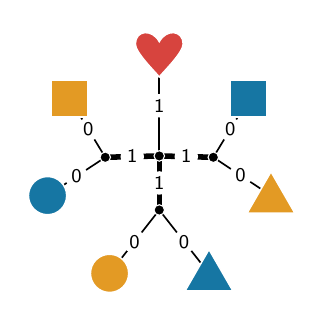
\begin{tikzpicture}[x=1.0cm,y=1.0cm,baseline=(current bounding box.center)]
\coordinate (v1) at (1.13770,0.90728);
\coordinate (v2) at (0.63137,-1.31106);
\coordinate (v3) at (-1.41868,-0.32381);
\coordinate (v4) at (-1.13770,0.90728);
\coordinate (v5) at (1.41868,-0.32381);
\coordinate (v6) at (-0.63137,-1.31106);
\coordinate (v7) at (0.00000,1.45517);
\coordinate (v8) at (0.68619,0.16311);
\coordinate (v9) at (0.00000,-0.50631);
\coordinate (v10) at (-0.68619,0.16311);
\coordinate (v11) at (0.00000,0.18009);
\draw[g2tree internal] (v8)--(v11);
\draw[g2tree internal] (v9)--(v11);
\draw[g2tree internal] (v10)--(v11);
\draw[g2tree pendant] (v1)--(v8);
\draw[g2tree pendant] (v2)--(v9);
\draw[g2tree pendant] (v3)--(v10);
\draw[g2tree pendant] (v4)--(v10);
\draw[g2tree pendant] (v5)--(v8);
\draw[g2tree pendant] (v6)--(v9);
\draw[g2tree pendant] (v7)--(v11);
\node[g2tree weight,font={\sffamily\fontsize{7.5}{8}\selectfont}] at (0.34309,0.17160) {1};
\node[g2tree weight,font={\sffamily\fontsize{7.5}{8}\selectfont}] at (0.00000,-0.16311) {1};
\node[g2tree weight,font={\sffamily\fontsize{7.5}{8}\selectfont}] at (-0.34309,0.17160) {1};
\node[g2tree weight,font={\sffamily\fontsize{7.5}{8}\selectfont}] at (0.90066,0.51659) {0};
\node[g2tree weight,font={\sffamily\fontsize{7.5}{8}\selectfont}] at (0.31569,-0.90869) {0};
\node[g2tree weight,font={\sffamily\fontsize{7.5}{8}\selectfont}] at (-1.05244,-0.08035) {0};
\node[g2tree weight,font={\sffamily\fontsize{7.5}{8}\selectfont}] at (-0.90066,0.51659) {0};
\node[g2tree weight,font={\sffamily\fontsize{7.5}{8}\selectfont}] at (1.03255,-0.06713) {0};
\node[g2tree weight,font={\sffamily\fontsize{7.5}{8}\selectfont}] at (-0.31569,-0.90869) {0};
\node[g2tree weight,font={\sffamily\fontsize{7.5}{8}\selectfont}] at (0.00000,0.81763) {1};
\node[g2tree vertex] at (v8) {};
\node[g2tree vertex] at (v9) {};
\node[g2tree vertex] at (v10) {};
\node[g2tree vertex] at (v11) {};
\node[g2tree dark,rectangle,minimum size=4.657500000000001mm,font={\sffamily\fontsize{9}{9}\selectfont\bfseries}] at (v1) {};
\begin{scope}[shift={(v2)},scale=1.0125000000000002,transform shape]
\path[fill=g2TaxonBlue,draw=white,line width=.55pt,line join=round] (0mm,3.0mm)--(-3.0mm,-2.2mm)--(3.0mm,-2.2mm)--cycle;
\end{scope}
\node[g2tree dark,circle,minimum size=4.86mm,font={\sffamily\fontsize{9}{9}\selectfont\bfseries}] at (v3) {};
\node[g2tree light,rectangle,minimum size=4.657500000000001mm,font={\sffamily\fontsize{9}{9}\selectfont\bfseries}] at (v4) {};
\begin{scope}[shift={(v5)},scale=1.0125000000000002,transform shape]
\path[fill=g2TaxonYellow,draw=white,line width=.55pt,line join=round] (0mm,3.0mm)--(-3.0mm,-2.2mm)--(3.0mm,-2.2mm)--cycle;
\end{scope}
\node[g2tree light,circle,minimum size=4.86mm,font={\sffamily\fontsize{9}{9}\selectfont\bfseries}] at (v6) {};
\begin{scope}[shift={(v7)},scale=1.0125000000000002,transform shape]
\path[fill=g2HeartRed,draw=white,line width=.55pt]
  (0mm,-2.7mm)..controls(-.45mm,-2.1mm)and(-3.0mm,.35mm)..(-3.0mm,1.45mm)
  ..controls(-3.0mm,3.2mm)and(-.9mm,3.4mm)..(0mm,1.75mm)
  ..controls(.9mm,3.4mm)and(3.0mm,3.2mm)..(3.0mm,1.45mm)
  ..controls(3.0mm,.35mm)and(.45mm,-2.1mm)..(0mm,-2.7mm)--cycle;
\end{scope}
\end{tikzpicture}
\endgroup
\par}
\end{minipage}
 & 
\begin{minipage}[t]{\linewidth}
\noindent\textcolor{g2TreeRule}{\rule{\linewidth}{1pt}}\par
\noindent\textcolor[HTML]{000000}{\smash[b]{\textpdfrender{TextRenderingMode=FillStroke,LineWidth=.5pt}{\Large\bfseries\boldmath \oldstylenums{22}}{\large(12)}}}\par
\vskip -2.5mm
{\centering
\begingroup
\definecolor{g2TaxonBlue}{HTML}{1676A3}
\definecolor{g2TaxonYellow}{HTML}{E39A24}
\definecolor{g2HeartRed}{HTML}{D7443E}
\tikzset{
  g2tree pendant/.style={draw=black,line width=.6pt,line cap=round},
  g2tree internal/.style={draw=black,line width=2pt,line cap=round},
  g2tree vertex/.style={circle,fill=black,draw=white,line width=.4pt,inner sep=0pt,minimum size=3.8pt},
  g2tree dark/.style={fill=g2TaxonBlue,draw=white,line width=.55pt,text=white,inner sep=0pt},
  g2tree light/.style={fill=g2TaxonYellow,draw=white,line width=.55pt,text=white,inner sep=0pt},
  g2tree weight/.style={circle,fill=white,draw=none,text=black,inner sep=.15pt,minimum size=8.5pt},
  g2tree aligned pendant/.style={fill=white,text=black,inner sep=.7pt,sloped,above=1pt,font={\sffamily\fontsize{7.5}{8}\selectfont}},
  g2tree aligned internal/.style={fill=white,text=black,inner sep=1pt,sloped,above=1pt,font={\sffamily\fontsize{7.5}{8}\selectfont\bfseries}},
}
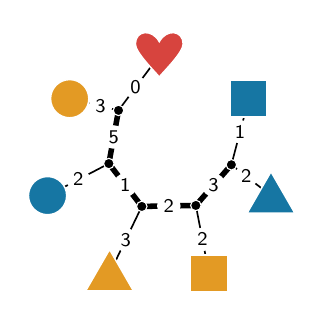
\begin{tikzpicture}[x=1.0cm,y=1.0cm,baseline=(current bounding box.center)]
\coordinate (v1) at (1.13770,0.90728);
\coordinate (v2) at (1.41868,-0.32381);
\coordinate (v3) at (-1.41868,-0.32381);
\coordinate (v4) at (0.63137,-1.31106);
\coordinate (v5) at (-0.63137,-1.31106);
\coordinate (v6) at (-1.13770,0.90728);
\coordinate (v7) at (0.00000,1.45517);
\coordinate (v8) at (-0.51766,0.75848);
\coordinate (v9) at (0.91576,0.06818);
\coordinate (v10) at (0.46431,-0.44886);
\coordinate (v11) at (-0.64042,0.08315);
\coordinate (v12) at (-0.22199,-0.46096);
\draw[g2tree internal] (v8)--(v11);
\draw[g2tree internal] (v9)--(v10);
\draw[g2tree internal] (v10)--(v12);
\draw[g2tree internal] (v11)--(v12);
\draw[g2tree pendant] (v1)--(v9);
\draw[g2tree pendant] (v2)--(v9);
\draw[g2tree pendant] (v3)--(v11);
\draw[g2tree pendant] (v4)--(v10);
\draw[g2tree pendant] (v5)--(v12);
\draw[g2tree pendant] (v6)--(v8);
\draw[g2tree pendant] (v7)--(v8);
\node[g2tree weight,font={\sffamily\fontsize{7.5}{8}\selectfont}] at (-0.57904,0.42082) {5};
\node[g2tree weight,font={\sffamily\fontsize{7.5}{8}\selectfont}] at (0.69004,-0.19034) {3};
\node[g2tree weight,font={\sffamily\fontsize{7.5}{8}\selectfont}] at (0.12116,-0.45491) {2};
\node[g2tree weight,font={\sffamily\fontsize{7.5}{8}\selectfont}] at (-0.43120,-0.18890) {1};
\node[g2tree weight,font={\sffamily\fontsize{7.5}{8}\selectfont}] at (1.02673,0.48773) {1};
\node[g2tree weight,font={\sffamily\fontsize{7.5}{8}\selectfont}] at (1.10436,-0.07881) {2};
\node[g2tree weight,font={\sffamily\fontsize{7.5}{8}\selectfont}] at (-1.02955,-0.12033) {2};
\node[g2tree weight,font={\sffamily\fontsize{7.5}{8}\selectfont}] at (0.54784,-0.87996) {2};
\node[g2tree weight,font={\sffamily\fontsize{7.5}{8}\selectfont}] at (-0.42668,-0.88601) {3};
\node[g2tree weight,font={\sffamily\fontsize{7.5}{8}\selectfont}] at (-0.74591,0.81326) {3};
\node[g2tree weight,font={\sffamily\fontsize{7.5}{8}\selectfont}] at (-0.30069,1.05049) {0};
\node[g2tree vertex] at (v8) {};
\node[g2tree vertex] at (v9) {};
\node[g2tree vertex] at (v10) {};
\node[g2tree vertex] at (v11) {};
\node[g2tree vertex] at (v12) {};
\node[g2tree dark,rectangle,minimum size=4.657500000000001mm,font={\sffamily\fontsize{9}{9}\selectfont\bfseries}] at (v1) {};
\begin{scope}[shift={(v2)},scale=1.0125000000000002,transform shape]
\path[fill=g2TaxonBlue,draw=white,line width=.55pt,line join=round] (0mm,3.0mm)--(-3.0mm,-2.2mm)--(3.0mm,-2.2mm)--cycle;
\end{scope}
\node[g2tree dark,circle,minimum size=4.86mm,font={\sffamily\fontsize{9}{9}\selectfont\bfseries}] at (v3) {};
\node[g2tree light,rectangle,minimum size=4.657500000000001mm,font={\sffamily\fontsize{9}{9}\selectfont\bfseries}] at (v4) {};
\begin{scope}[shift={(v5)},scale=1.0125000000000002,transform shape]
\path[fill=g2TaxonYellow,draw=white,line width=.55pt,line join=round] (0mm,3.0mm)--(-3.0mm,-2.2mm)--(3.0mm,-2.2mm)--cycle;
\end{scope}
\node[g2tree light,circle,minimum size=4.86mm,font={\sffamily\fontsize{9}{9}\selectfont\bfseries}] at (v6) {};
\begin{scope}[shift={(v7)},scale=1.0125000000000002,transform shape]
\path[fill=g2HeartRed,draw=white,line width=.55pt]
  (0mm,-2.7mm)..controls(-.45mm,-2.1mm)and(-3.0mm,.35mm)..(-3.0mm,1.45mm)
  ..controls(-3.0mm,3.2mm)and(-.9mm,3.4mm)..(0mm,1.75mm)
  ..controls(.9mm,3.4mm)and(3.0mm,3.2mm)..(3.0mm,1.45mm)
  ..controls(3.0mm,.35mm)and(.45mm,-2.1mm)..(0mm,-2.7mm)--cycle;
\end{scope}
\end{tikzpicture}
\endgroup
\par}
\end{minipage}
 & 
\begin{minipage}[t]{\linewidth}
\noindent\textcolor{g2TreeRule}{\rule{\linewidth}{1pt}}\par
\noindent\textcolor[HTML]{000000}{\smash[b]{\textpdfrender{TextRenderingMode=FillStroke,LineWidth=.5pt}{\Large\bfseries\boldmath \oldstylenums{23}}{\large(12)}}}\par
\vskip -2.5mm
{\centering
\begingroup
\definecolor{g2TaxonBlue}{HTML}{1676A3}
\definecolor{g2TaxonYellow}{HTML}{E39A24}
\definecolor{g2HeartRed}{HTML}{D7443E}
\tikzset{
  g2tree pendant/.style={draw=black,line width=.6pt,line cap=round},
  g2tree internal/.style={draw=black,line width=2pt,line cap=round},
  g2tree vertex/.style={circle,fill=black,draw=white,line width=.4pt,inner sep=0pt,minimum size=3.8pt},
  g2tree dark/.style={fill=g2TaxonBlue,draw=white,line width=.55pt,text=white,inner sep=0pt},
  g2tree light/.style={fill=g2TaxonYellow,draw=white,line width=.55pt,text=white,inner sep=0pt},
  g2tree weight/.style={circle,fill=white,draw=none,text=black,inner sep=.15pt,minimum size=8.5pt},
  g2tree aligned pendant/.style={fill=white,text=black,inner sep=.7pt,sloped,above=1pt,font={\sffamily\fontsize{7.5}{8}\selectfont}},
  g2tree aligned internal/.style={fill=white,text=black,inner sep=1pt,sloped,above=1pt,font={\sffamily\fontsize{7.5}{8}\selectfont\bfseries}},
}
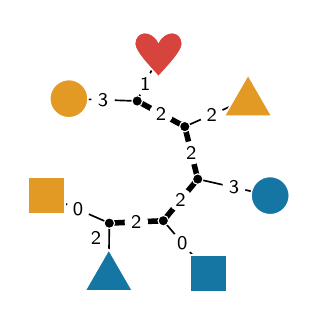
\begin{tikzpicture}[x=1.0cm,y=1.0cm,baseline=(current bounding box.center)]
\coordinate (v1) at (0.63137,-1.31106);
\coordinate (v2) at (-0.63137,-1.31106);
\coordinate (v3) at (1.41868,-0.32381);
\coordinate (v4) at (-1.41868,-0.32381);
\coordinate (v5) at (1.13770,0.90728);
\coordinate (v6) at (-1.13770,0.90728);
\coordinate (v7) at (0.00000,1.45517);
\coordinate (v8) at (-0.62428,-0.67346);
\coordinate (v9) at (0.06144,-0.64287);
\coordinate (v10) at (0.49880,-0.11385);
\coordinate (v11) at (0.33429,0.55255);
\coordinate (v12) at (-0.27025,0.87763);
\draw[g2tree internal] (v8)--(v9);
\draw[g2tree internal] (v9)--(v10);
\draw[g2tree internal] (v10)--(v11);
\draw[g2tree internal] (v11)--(v12);
\draw[g2tree pendant] (v1)--(v9);
\draw[g2tree pendant] (v2)--(v8);
\draw[g2tree pendant] (v3)--(v10);
\draw[g2tree pendant] (v4)--(v8);
\draw[g2tree pendant] (v5)--(v11);
\draw[g2tree pendant] (v6)--(v12);
\draw[g2tree pendant] (v7)--(v12);
\node[g2tree weight,font={\sffamily\fontsize{7.5}{8}\selectfont}] at (-0.28142,-0.65816) {2};
\node[g2tree weight,font={\sffamily\fontsize{7.5}{8}\selectfont}] at (0.28012,-0.37836) {2};
\node[g2tree weight,font={\sffamily\fontsize{7.5}{8}\selectfont}] at (0.41654,0.21935) {2};
\node[g2tree weight,font={\sffamily\fontsize{7.5}{8}\selectfont}] at (0.03202,0.71509) {2};
\node[g2tree weight,font={\sffamily\fontsize{7.5}{8}\selectfont}] at (0.30366,-0.92685) {0};
\node[g2tree weight,font={\sffamily\fontsize{7.5}{8}\selectfont}] at (-0.79334,-0.86288) {2};
\node[g2tree weight,font={\sffamily\fontsize{7.5}{8}\selectfont}] at (0.95874,-0.21883) {3};
\node[g2tree weight,font={\sffamily\fontsize{7.5}{8}\selectfont}] at (-1.02148,-0.49863) {0};
\node[g2tree weight,font={\sffamily\fontsize{7.5}{8}\selectfont}] at (0.67574,0.70331) {2};
\node[g2tree weight,font={\sffamily\fontsize{7.5}{8}\selectfont}] at (-0.70397,0.89246) {3};
\node[g2tree weight,font={\sffamily\fontsize{7.5}{8}\selectfont}] at (-0.16891,1.09421) {1};
\node[g2tree vertex] at (v8) {};
\node[g2tree vertex] at (v9) {};
\node[g2tree vertex] at (v10) {};
\node[g2tree vertex] at (v11) {};
\node[g2tree vertex] at (v12) {};
\node[g2tree dark,rectangle,minimum size=4.657500000000001mm,font={\sffamily\fontsize{9}{9}\selectfont\bfseries}] at (v1) {};
\begin{scope}[shift={(v2)},scale=1.0125000000000002,transform shape]
\path[fill=g2TaxonBlue,draw=white,line width=.55pt,line join=round] (0mm,3.0mm)--(-3.0mm,-2.2mm)--(3.0mm,-2.2mm)--cycle;
\end{scope}
\node[g2tree dark,circle,minimum size=4.86mm,font={\sffamily\fontsize{9}{9}\selectfont\bfseries}] at (v3) {};
\node[g2tree light,rectangle,minimum size=4.657500000000001mm,font={\sffamily\fontsize{9}{9}\selectfont\bfseries}] at (v4) {};
\begin{scope}[shift={(v5)},scale=1.0125000000000002,transform shape]
\path[fill=g2TaxonYellow,draw=white,line width=.55pt,line join=round] (0mm,3.0mm)--(-3.0mm,-2.2mm)--(3.0mm,-2.2mm)--cycle;
\end{scope}
\node[g2tree light,circle,minimum size=4.86mm,font={\sffamily\fontsize{9}{9}\selectfont\bfseries}] at (v6) {};
\begin{scope}[shift={(v7)},scale=1.0125000000000002,transform shape]
\path[fill=g2HeartRed,draw=white,line width=.55pt]
  (0mm,-2.7mm)..controls(-.45mm,-2.1mm)and(-3.0mm,.35mm)..(-3.0mm,1.45mm)
  ..controls(-3.0mm,3.2mm)and(-.9mm,3.4mm)..(0mm,1.75mm)
  ..controls(.9mm,3.4mm)and(3.0mm,3.2mm)..(3.0mm,1.45mm)
  ..controls(3.0mm,.35mm)and(.45mm,-2.1mm)..(0mm,-2.7mm)--cycle;
\end{scope}
\end{tikzpicture}
\endgroup
\par}
\end{minipage}
\\\noalign{\vskip 0.22cm}
\begin{minipage}[t]{\linewidth}
\noindent\textcolor{g2TreeRule}{\rule{\linewidth}{1pt}}\par
\noindent\textcolor[HTML]{000000}{\smash[b]{\textpdfrender{TextRenderingMode=FillStroke,LineWidth=.5pt}{\Large\bfseries\boldmath \oldstylenums{24}}{\large(12)}}}\par
\vskip -2.5mm
{\centering
\begingroup
\definecolor{g2TaxonBlue}{HTML}{1676A3}
\definecolor{g2TaxonYellow}{HTML}{E39A24}
\definecolor{g2HeartRed}{HTML}{D7443E}
\tikzset{
  g2tree pendant/.style={draw=black,line width=.6pt,line cap=round},
  g2tree internal/.style={draw=black,line width=2pt,line cap=round},
  g2tree vertex/.style={circle,fill=black,draw=white,line width=.4pt,inner sep=0pt,minimum size=3.8pt},
  g2tree dark/.style={fill=g2TaxonBlue,draw=white,line width=.55pt,text=white,inner sep=0pt},
  g2tree light/.style={fill=g2TaxonYellow,draw=white,line width=.55pt,text=white,inner sep=0pt},
  g2tree weight/.style={circle,fill=white,draw=none,text=black,inner sep=.15pt,minimum size=8.5pt},
  g2tree aligned pendant/.style={fill=white,text=black,inner sep=.7pt,sloped,above=1pt,font={\sffamily\fontsize{7.5}{8}\selectfont}},
  g2tree aligned internal/.style={fill=white,text=black,inner sep=1pt,sloped,above=1pt,font={\sffamily\fontsize{7.5}{8}\selectfont\bfseries}},
}
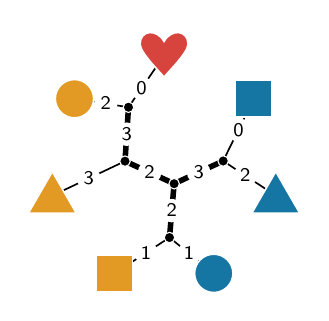
\begin{tikzpicture}[x=1.0cm,y=1.0cm,baseline=(current bounding box.center)]
\coordinate (v1) at (1.13770,0.90728);
\coordinate (v2) at (1.41868,-0.32381);
\coordinate (v3) at (0.63137,-1.31106);
\coordinate (v4) at (-0.63137,-1.31106);
\coordinate (v5) at (-1.41868,-0.32381);
\coordinate (v6) at (-1.13770,0.90728);
\coordinate (v7) at (0.00000,1.45517);
\coordinate (v8) at (-0.45173,0.79874);
\coordinate (v9) at (0.75079,0.11610);
\coordinate (v10) at (0.06894,-0.85624);
\coordinate (v11) at (-0.49596,0.11377);
\coordinate (v12) at (0.12795,-0.17238);
\draw[g2tree internal] (v8)--(v11);
\draw[g2tree internal] (v9)--(v12);
\draw[g2tree internal] (v10)--(v12);
\draw[g2tree internal] (v11)--(v12);
\draw[g2tree pendant] (v1)--(v9);
\draw[g2tree pendant] (v2)--(v9);
\draw[g2tree pendant] (v3)--(v10);
\draw[g2tree pendant] (v4)--(v10);
\draw[g2tree pendant] (v5)--(v11);
\draw[g2tree pendant] (v6)--(v8);
\draw[g2tree pendant] (v7)--(v8);
\node[g2tree weight,font={\sffamily\fontsize{7.5}{8}\selectfont}] at (-0.47384,0.45626) {3};
\node[g2tree weight,font={\sffamily\fontsize{7.5}{8}\selectfont}] at (0.43937,-0.02814) {3};
\node[g2tree weight,font={\sffamily\fontsize{7.5}{8}\selectfont}] at (0.09845,-0.51431) {2};
\node[g2tree weight,font={\sffamily\fontsize{7.5}{8}\selectfont}] at (-0.18400,-0.02930) {2};
\node[g2tree weight,font={\sffamily\fontsize{7.5}{8}\selectfont}] at (0.94424,0.51169) {0};
\node[g2tree weight,font={\sffamily\fontsize{7.5}{8}\selectfont}] at (1.03147,-0.06876) {2};
\node[g2tree weight,font={\sffamily\fontsize{7.5}{8}\selectfont}] at (0.31808,-1.05771) {1};
\node[g2tree weight,font={\sffamily\fontsize{7.5}{8}\selectfont}] at (-0.22869,-1.04954) {1};
\node[g2tree weight,font={\sffamily\fontsize{7.5}{8}\selectfont}] at (-0.95732,-0.10502) {3};
\node[g2tree weight,font={\sffamily\fontsize{7.5}{8}\selectfont}] at (-0.73973,0.84431) {2};
\node[g2tree weight,font={\sffamily\fontsize{7.5}{8}\selectfont}] at (-0.28581,1.03984) {0};
\node[g2tree vertex] at (v8) {};
\node[g2tree vertex] at (v9) {};
\node[g2tree vertex] at (v10) {};
\node[g2tree vertex] at (v11) {};
\node[g2tree vertex] at (v12) {};
\node[g2tree dark,rectangle,minimum size=4.657500000000001mm,font={\sffamily\fontsize{9}{9}\selectfont\bfseries}] at (v1) {};
\begin{scope}[shift={(v2)},scale=1.0125000000000002,transform shape]
\path[fill=g2TaxonBlue,draw=white,line width=.55pt,line join=round] (0mm,3.0mm)--(-3.0mm,-2.2mm)--(3.0mm,-2.2mm)--cycle;
\end{scope}
\node[g2tree dark,circle,minimum size=4.86mm,font={\sffamily\fontsize{9}{9}\selectfont\bfseries}] at (v3) {};
\node[g2tree light,rectangle,minimum size=4.657500000000001mm,font={\sffamily\fontsize{9}{9}\selectfont\bfseries}] at (v4) {};
\begin{scope}[shift={(v5)},scale=1.0125000000000002,transform shape]
\path[fill=g2TaxonYellow,draw=white,line width=.55pt,line join=round] (0mm,3.0mm)--(-3.0mm,-2.2mm)--(3.0mm,-2.2mm)--cycle;
\end{scope}
\node[g2tree light,circle,minimum size=4.86mm,font={\sffamily\fontsize{9}{9}\selectfont\bfseries}] at (v6) {};
\begin{scope}[shift={(v7)},scale=1.0125000000000002,transform shape]
\path[fill=g2HeartRed,draw=white,line width=.55pt]
  (0mm,-2.7mm)..controls(-.45mm,-2.1mm)and(-3.0mm,.35mm)..(-3.0mm,1.45mm)
  ..controls(-3.0mm,3.2mm)and(-.9mm,3.4mm)..(0mm,1.75mm)
  ..controls(.9mm,3.4mm)and(3.0mm,3.2mm)..(3.0mm,1.45mm)
  ..controls(3.0mm,.35mm)and(.45mm,-2.1mm)..(0mm,-2.7mm)--cycle;
\end{scope}
\end{tikzpicture}
\endgroup
\par}
\end{minipage}
 & 
\begin{minipage}[t]{\linewidth}
\noindent\textcolor{g2TreeRule}{\rule{\linewidth}{1pt}}\par
\noindent\textcolor[HTML]{000000}{\smash[b]{\textpdfrender{TextRenderingMode=FillStroke,LineWidth=.5pt}{\Large\bfseries\boldmath \oldstylenums{25}}{\large(12)}}}\par
\vskip -2.5mm
{\centering
\begingroup
\definecolor{g2TaxonBlue}{HTML}{1676A3}
\definecolor{g2TaxonYellow}{HTML}{E39A24}
\definecolor{g2HeartRed}{HTML}{D7443E}
\tikzset{
  g2tree pendant/.style={draw=black,line width=.6pt,line cap=round},
  g2tree internal/.style={draw=black,line width=2pt,line cap=round},
  g2tree vertex/.style={circle,fill=black,draw=white,line width=.4pt,inner sep=0pt,minimum size=3.8pt},
  g2tree dark/.style={fill=g2TaxonBlue,draw=white,line width=.55pt,text=white,inner sep=0pt},
  g2tree light/.style={fill=g2TaxonYellow,draw=white,line width=.55pt,text=white,inner sep=0pt},
  g2tree weight/.style={circle,fill=white,draw=none,text=black,inner sep=.15pt,minimum size=8.5pt},
  g2tree aligned pendant/.style={fill=white,text=black,inner sep=.7pt,sloped,above=1pt,font={\sffamily\fontsize{7.5}{8}\selectfont}},
  g2tree aligned internal/.style={fill=white,text=black,inner sep=1pt,sloped,above=1pt,font={\sffamily\fontsize{7.5}{8}\selectfont\bfseries}},
}
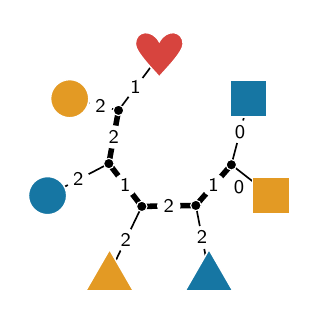
\begin{tikzpicture}[x=1.0cm,y=1.0cm,baseline=(current bounding box.center)]
\coordinate (v1) at (1.13770,0.90728);
\coordinate (v2) at (0.63137,-1.31106);
\coordinate (v3) at (-1.41868,-0.32381);
\coordinate (v4) at (1.41868,-0.32381);
\coordinate (v5) at (-0.63137,-1.31106);
\coordinate (v6) at (-1.13770,0.90728);
\coordinate (v7) at (0.00000,1.45517);
\coordinate (v8) at (-0.51766,0.75848);
\coordinate (v9) at (0.91576,0.06818);
\coordinate (v10) at (0.46431,-0.44886);
\coordinate (v11) at (-0.64042,0.08315);
\coordinate (v12) at (-0.22199,-0.46096);
\draw[g2tree internal] (v8)--(v11);
\draw[g2tree internal] (v9)--(v10);
\draw[g2tree internal] (v10)--(v12);
\draw[g2tree internal] (v11)--(v12);
\draw[g2tree pendant] (v1)--(v9);
\draw[g2tree pendant] (v2)--(v10);
\draw[g2tree pendant] (v3)--(v11);
\draw[g2tree pendant] (v4)--(v9);
\draw[g2tree pendant] (v5)--(v12);
\draw[g2tree pendant] (v6)--(v8);
\draw[g2tree pendant] (v7)--(v8);
\node[g2tree weight,font={\sffamily\fontsize{7.5}{8}\selectfont}] at (-0.57904,0.42082) {2};
\node[g2tree weight,font={\sffamily\fontsize{7.5}{8}\selectfont}] at (0.69004,-0.19034) {1};
\node[g2tree weight,font={\sffamily\fontsize{7.5}{8}\selectfont}] at (0.12116,-0.45491) {2};
\node[g2tree weight,font={\sffamily\fontsize{7.5}{8}\selectfont}] at (-0.43120,-0.18890) {1};
\node[g2tree weight,font={\sffamily\fontsize{7.5}{8}\selectfont}] at (1.02673,0.48773) {0};
\node[g2tree weight,font={\sffamily\fontsize{7.5}{8}\selectfont}] at (0.54317,-0.85586) {2};
\node[g2tree weight,font={\sffamily\fontsize{7.5}{8}\selectfont}] at (-1.02955,-0.12033) {2};
\node[g2tree weight,font={\sffamily\fontsize{7.5}{8}\selectfont}] at (1.01430,-0.22028) {0};
\node[g2tree weight,font={\sffamily\fontsize{7.5}{8}\selectfont}] at (-0.42668,-0.88601) {2};
\node[g2tree weight,font={\sffamily\fontsize{7.5}{8}\selectfont}] at (-0.74591,0.81326) {2};
\node[g2tree weight,font={\sffamily\fontsize{7.5}{8}\selectfont}] at (-0.30069,1.05049) {1};
\node[g2tree vertex] at (v8) {};
\node[g2tree vertex] at (v9) {};
\node[g2tree vertex] at (v10) {};
\node[g2tree vertex] at (v11) {};
\node[g2tree vertex] at (v12) {};
\node[g2tree dark,rectangle,minimum size=4.657500000000001mm,font={\sffamily\fontsize{9}{9}\selectfont\bfseries}] at (v1) {};
\begin{scope}[shift={(v2)},scale=1.0125000000000002,transform shape]
\path[fill=g2TaxonBlue,draw=white,line width=.55pt,line join=round] (0mm,3.0mm)--(-3.0mm,-2.2mm)--(3.0mm,-2.2mm)--cycle;
\end{scope}
\node[g2tree dark,circle,minimum size=4.86mm,font={\sffamily\fontsize{9}{9}\selectfont\bfseries}] at (v3) {};
\node[g2tree light,rectangle,minimum size=4.657500000000001mm,font={\sffamily\fontsize{9}{9}\selectfont\bfseries}] at (v4) {};
\begin{scope}[shift={(v5)},scale=1.0125000000000002,transform shape]
\path[fill=g2TaxonYellow,draw=white,line width=.55pt,line join=round] (0mm,3.0mm)--(-3.0mm,-2.2mm)--(3.0mm,-2.2mm)--cycle;
\end{scope}
\node[g2tree light,circle,minimum size=4.86mm,font={\sffamily\fontsize{9}{9}\selectfont\bfseries}] at (v6) {};
\begin{scope}[shift={(v7)},scale=1.0125000000000002,transform shape]
\path[fill=g2HeartRed,draw=white,line width=.55pt]
  (0mm,-2.7mm)..controls(-.45mm,-2.1mm)and(-3.0mm,.35mm)..(-3.0mm,1.45mm)
  ..controls(-3.0mm,3.2mm)and(-.9mm,3.4mm)..(0mm,1.75mm)
  ..controls(.9mm,3.4mm)and(3.0mm,3.2mm)..(3.0mm,1.45mm)
  ..controls(3.0mm,.35mm)and(.45mm,-2.1mm)..(0mm,-2.7mm)--cycle;
\end{scope}
\end{tikzpicture}
\endgroup
\par}
\end{minipage}
 & 
\begin{minipage}[t]{\linewidth}
\noindent\textcolor{g2TreeRule}{\rule{\linewidth}{1pt}}\par
\noindent\textcolor[HTML]{000000}{\smash[b]{\textpdfrender{TextRenderingMode=FillStroke,LineWidth=.5pt}{\Large\bfseries\boldmath \oldstylenums{26}}{\large(12)}}}\par
\vskip -2.5mm
{\centering
\begingroup
\definecolor{g2TaxonBlue}{HTML}{1676A3}
\definecolor{g2TaxonYellow}{HTML}{E39A24}
\definecolor{g2HeartRed}{HTML}{D7443E}
\tikzset{
  g2tree pendant/.style={draw=black,line width=.6pt,line cap=round},
  g2tree internal/.style={draw=black,line width=2pt,line cap=round},
  g2tree vertex/.style={circle,fill=black,draw=white,line width=.4pt,inner sep=0pt,minimum size=3.8pt},
  g2tree dark/.style={fill=g2TaxonBlue,draw=white,line width=.55pt,text=white,inner sep=0pt},
  g2tree light/.style={fill=g2TaxonYellow,draw=white,line width=.55pt,text=white,inner sep=0pt},
  g2tree weight/.style={circle,fill=white,draw=none,text=black,inner sep=.15pt,minimum size=8.5pt},
  g2tree aligned pendant/.style={fill=white,text=black,inner sep=.7pt,sloped,above=1pt,font={\sffamily\fontsize{7.5}{8}\selectfont}},
  g2tree aligned internal/.style={fill=white,text=black,inner sep=1pt,sloped,above=1pt,font={\sffamily\fontsize{7.5}{8}\selectfont\bfseries}},
}
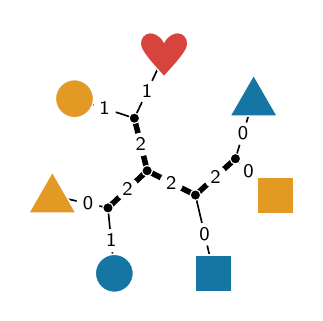
\begin{tikzpicture}[x=1.0cm,y=1.0cm,baseline=(current bounding box.center)]
\coordinate (v1) at (0.63137,-1.31106);
\coordinate (v2) at (1.13770,0.90728);
\coordinate (v3) at (-0.63137,-1.31106);
\coordinate (v4) at (1.41868,-0.32381);
\coordinate (v5) at (-1.41868,-0.32381);
\coordinate (v6) at (-1.13770,0.90728);
\coordinate (v7) at (0.00000,1.45517);
\coordinate (v8) at (0.90613,0.14484);
\coordinate (v9) at (0.39817,-0.31682);
\coordinate (v10) at (-0.71242,-0.47995);
\coordinate (v11) at (-0.37733,0.65938);
\coordinate (v12) at (-0.21455,-0.00744);
\draw[g2tree internal] (v8)--(v9);
\draw[g2tree internal] (v9)--(v12);
\draw[g2tree internal] (v10)--(v12);
\draw[g2tree internal] (v11)--(v12);
\draw[g2tree pendant] (v1)--(v9);
\draw[g2tree pendant] (v2)--(v8);
\draw[g2tree pendant] (v3)--(v10);
\draw[g2tree pendant] (v4)--(v8);
\draw[g2tree pendant] (v5)--(v10);
\draw[g2tree pendant] (v6)--(v11);
\draw[g2tree pendant] (v7)--(v11);
\node[g2tree weight,font={\sffamily\fontsize{7.5}{8}\selectfont}] at (0.65215,-0.08599) {2};
\node[g2tree weight,font={\sffamily\fontsize{7.5}{8}\selectfont}] at (0.09181,-0.16213) {2};
\node[g2tree weight,font={\sffamily\fontsize{7.5}{8}\selectfont}] at (-0.46348,-0.24370) {2};
\node[g2tree weight,font={\sffamily\fontsize{7.5}{8}\selectfont}] at (-0.29594,0.32597) {2};
\node[g2tree weight,font={\sffamily\fontsize{7.5}{8}\selectfont}] at (0.51477,-0.81394) {0};
\node[g2tree weight,font={\sffamily\fontsize{7.5}{8}\selectfont}] at (1.00295,0.46363) {0};
\node[g2tree weight,font={\sffamily\fontsize{7.5}{8}\selectfont}] at (-0.67190,-0.89551) {1};
\node[g2tree weight,font={\sffamily\fontsize{7.5}{8}\selectfont}] at (1.07271,-0.00747) {0};
\node[g2tree weight,font={\sffamily\fontsize{7.5}{8}\selectfont}] at (-0.96595,-0.42390) {0};
\node[g2tree weight,font={\sffamily\fontsize{7.5}{8}\selectfont}] at (-0.75463,0.78239) {1};
\node[g2tree weight,font={\sffamily\fontsize{7.5}{8}\selectfont}] at (-0.21600,0.99962) {1};
\node[g2tree vertex] at (v8) {};
\node[g2tree vertex] at (v9) {};
\node[g2tree vertex] at (v10) {};
\node[g2tree vertex] at (v11) {};
\node[g2tree vertex] at (v12) {};
\node[g2tree dark,rectangle,minimum size=4.657500000000001mm,font={\sffamily\fontsize{9}{9}\selectfont\bfseries}] at (v1) {};
\begin{scope}[shift={(v2)},scale=1.0125000000000002,transform shape]
\path[fill=g2TaxonBlue,draw=white,line width=.55pt,line join=round] (0mm,3.0mm)--(-3.0mm,-2.2mm)--(3.0mm,-2.2mm)--cycle;
\end{scope}
\node[g2tree dark,circle,minimum size=4.86mm,font={\sffamily\fontsize{9}{9}\selectfont\bfseries}] at (v3) {};
\node[g2tree light,rectangle,minimum size=4.657500000000001mm,font={\sffamily\fontsize{9}{9}\selectfont\bfseries}] at (v4) {};
\begin{scope}[shift={(v5)},scale=1.0125000000000002,transform shape]
\path[fill=g2TaxonYellow,draw=white,line width=.55pt,line join=round] (0mm,3.0mm)--(-3.0mm,-2.2mm)--(3.0mm,-2.2mm)--cycle;
\end{scope}
\node[g2tree light,circle,minimum size=4.86mm,font={\sffamily\fontsize{9}{9}\selectfont\bfseries}] at (v6) {};
\begin{scope}[shift={(v7)},scale=1.0125000000000002,transform shape]
\path[fill=g2HeartRed,draw=white,line width=.55pt]
  (0mm,-2.7mm)..controls(-.45mm,-2.1mm)and(-3.0mm,.35mm)..(-3.0mm,1.45mm)
  ..controls(-3.0mm,3.2mm)and(-.9mm,3.4mm)..(0mm,1.75mm)
  ..controls(.9mm,3.4mm)and(3.0mm,3.2mm)..(3.0mm,1.45mm)
  ..controls(3.0mm,.35mm)and(.45mm,-2.1mm)..(0mm,-2.7mm)--cycle;
\end{scope}
\end{tikzpicture}
\endgroup
\par}
\end{minipage}
\\\noalign{\vskip 0.22cm}
\begin{minipage}[t]{\linewidth}
\noindent\textcolor{g2TreeRule}{\rule{\linewidth}{1pt}}\par
\noindent\textcolor[HTML]{000000}{\smash[b]{\textpdfrender{TextRenderingMode=FillStroke,LineWidth=.5pt}{\Large\bfseries\boldmath \oldstylenums{27}}{\large(12)}}}\par
\vskip -2.5mm
{\centering
\begingroup
\definecolor{g2TaxonBlue}{HTML}{1676A3}
\definecolor{g2TaxonYellow}{HTML}{E39A24}
\definecolor{g2HeartRed}{HTML}{D7443E}
\tikzset{
  g2tree pendant/.style={draw=black,line width=.6pt,line cap=round},
  g2tree internal/.style={draw=black,line width=2pt,line cap=round},
  g2tree vertex/.style={circle,fill=black,draw=white,line width=.4pt,inner sep=0pt,minimum size=3.8pt},
  g2tree dark/.style={fill=g2TaxonBlue,draw=white,line width=.55pt,text=white,inner sep=0pt},
  g2tree light/.style={fill=g2TaxonYellow,draw=white,line width=.55pt,text=white,inner sep=0pt},
  g2tree weight/.style={circle,fill=white,draw=none,text=black,inner sep=.15pt,minimum size=8.5pt},
  g2tree aligned pendant/.style={fill=white,text=black,inner sep=.7pt,sloped,above=1pt,font={\sffamily\fontsize{7.5}{8}\selectfont}},
  g2tree aligned internal/.style={fill=white,text=black,inner sep=1pt,sloped,above=1pt,font={\sffamily\fontsize{7.5}{8}\selectfont\bfseries}},
}
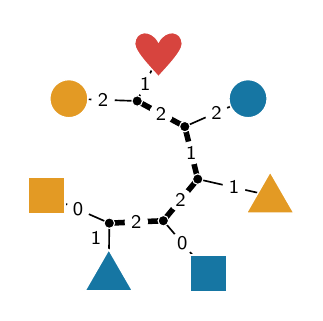
\begin{tikzpicture}[x=1.0cm,y=1.0cm,baseline=(current bounding box.center)]
\coordinate (v1) at (0.63137,-1.31106);
\coordinate (v2) at (-0.63137,-1.31106);
\coordinate (v3) at (1.13770,0.90728);
\coordinate (v4) at (-1.41868,-0.32381);
\coordinate (v5) at (1.41868,-0.32381);
\coordinate (v6) at (-1.13770,0.90728);
\coordinate (v7) at (0.00000,1.45517);
\coordinate (v8) at (-0.62428,-0.67346);
\coordinate (v9) at (0.06144,-0.64287);
\coordinate (v10) at (-0.27025,0.87763);
\coordinate (v11) at (0.33429,0.55255);
\coordinate (v12) at (0.49880,-0.11385);
\draw[g2tree internal] (v8)--(v9);
\draw[g2tree internal] (v9)--(v12);
\draw[g2tree internal] (v10)--(v11);
\draw[g2tree internal] (v11)--(v12);
\draw[g2tree pendant] (v1)--(v9);
\draw[g2tree pendant] (v2)--(v8);
\draw[g2tree pendant] (v3)--(v11);
\draw[g2tree pendant] (v4)--(v8);
\draw[g2tree pendant] (v5)--(v12);
\draw[g2tree pendant] (v6)--(v10);
\draw[g2tree pendant] (v7)--(v10);
\node[g2tree weight,font={\sffamily\fontsize{7.5}{8}\selectfont}] at (-0.28142,-0.65816) {2};
\node[g2tree weight,font={\sffamily\fontsize{7.5}{8}\selectfont}] at (0.28012,-0.37836) {2};
\node[g2tree weight,font={\sffamily\fontsize{7.5}{8}\selectfont}] at (0.03202,0.71509) {2};
\node[g2tree weight,font={\sffamily\fontsize{7.5}{8}\selectfont}] at (0.41654,0.21935) {1};
\node[g2tree weight,font={\sffamily\fontsize{7.5}{8}\selectfont}] at (0.30366,-0.92685) {0};
\node[g2tree weight,font={\sffamily\fontsize{7.5}{8}\selectfont}] at (-0.79334,-0.86288) {1};
\node[g2tree weight,font={\sffamily\fontsize{7.5}{8}\selectfont}] at (0.73599,0.72991) {2};
\node[g2tree weight,font={\sffamily\fontsize{7.5}{8}\selectfont}] at (-1.02148,-0.49863) {0};
\node[g2tree weight,font={\sffamily\fontsize{7.5}{8}\selectfont}] at (0.95874,-0.21883) {1};
\node[g2tree weight,font={\sffamily\fontsize{7.5}{8}\selectfont}] at (-0.70397,0.89246) {2};
\node[g2tree weight,font={\sffamily\fontsize{7.5}{8}\selectfont}] at (-0.16891,1.09421) {1};
\node[g2tree vertex] at (v8) {};
\node[g2tree vertex] at (v9) {};
\node[g2tree vertex] at (v10) {};
\node[g2tree vertex] at (v11) {};
\node[g2tree vertex] at (v12) {};
\node[g2tree dark,rectangle,minimum size=4.657500000000001mm,font={\sffamily\fontsize{9}{9}\selectfont\bfseries}] at (v1) {};
\begin{scope}[shift={(v2)},scale=1.0125000000000002,transform shape]
\path[fill=g2TaxonBlue,draw=white,line width=.55pt,line join=round] (0mm,3.0mm)--(-3.0mm,-2.2mm)--(3.0mm,-2.2mm)--cycle;
\end{scope}
\node[g2tree dark,circle,minimum size=4.86mm,font={\sffamily\fontsize{9}{9}\selectfont\bfseries}] at (v3) {};
\node[g2tree light,rectangle,minimum size=4.657500000000001mm,font={\sffamily\fontsize{9}{9}\selectfont\bfseries}] at (v4) {};
\begin{scope}[shift={(v5)},scale=1.0125000000000002,transform shape]
\path[fill=g2TaxonYellow,draw=white,line width=.55pt,line join=round] (0mm,3.0mm)--(-3.0mm,-2.2mm)--(3.0mm,-2.2mm)--cycle;
\end{scope}
\node[g2tree light,circle,minimum size=4.86mm,font={\sffamily\fontsize{9}{9}\selectfont\bfseries}] at (v6) {};
\begin{scope}[shift={(v7)},scale=1.0125000000000002,transform shape]
\path[fill=g2HeartRed,draw=white,line width=.55pt]
  (0mm,-2.7mm)..controls(-.45mm,-2.1mm)and(-3.0mm,.35mm)..(-3.0mm,1.45mm)
  ..controls(-3.0mm,3.2mm)and(-.9mm,3.4mm)..(0mm,1.75mm)
  ..controls(.9mm,3.4mm)and(3.0mm,3.2mm)..(3.0mm,1.45mm)
  ..controls(3.0mm,.35mm)and(.45mm,-2.1mm)..(0mm,-2.7mm)--cycle;
\end{scope}
\end{tikzpicture}
\endgroup
\par}
\end{minipage}
 & 
\begin{minipage}[t]{\linewidth}
\noindent\textcolor{g2TreeRule}{\rule{\linewidth}{1pt}}\par
\noindent\textcolor[HTML]{000000}{\smash[b]{\textpdfrender{TextRenderingMode=FillStroke,LineWidth=.5pt}{\Large\bfseries\boldmath \oldstylenums{28}}{\large(6)}}}\par
\vskip -2.5mm
{\centering
\begingroup
\definecolor{g2TaxonBlue}{HTML}{1676A3}
\definecolor{g2TaxonYellow}{HTML}{E39A24}
\definecolor{g2HeartRed}{HTML}{D7443E}
\tikzset{
  g2tree pendant/.style={draw=black,line width=.6pt,line cap=round},
  g2tree internal/.style={draw=black,line width=2pt,line cap=round},
  g2tree vertex/.style={circle,fill=black,draw=white,line width=.4pt,inner sep=0pt,minimum size=3.8pt},
  g2tree dark/.style={fill=g2TaxonBlue,draw=white,line width=.55pt,text=white,inner sep=0pt},
  g2tree light/.style={fill=g2TaxonYellow,draw=white,line width=.55pt,text=white,inner sep=0pt},
  g2tree weight/.style={circle,fill=white,draw=none,text=black,inner sep=.15pt,minimum size=8.5pt},
  g2tree aligned pendant/.style={fill=white,text=black,inner sep=.7pt,sloped,above=1pt,font={\sffamily\fontsize{7.5}{8}\selectfont}},
  g2tree aligned internal/.style={fill=white,text=black,inner sep=1pt,sloped,above=1pt,font={\sffamily\fontsize{7.5}{8}\selectfont\bfseries}},
}
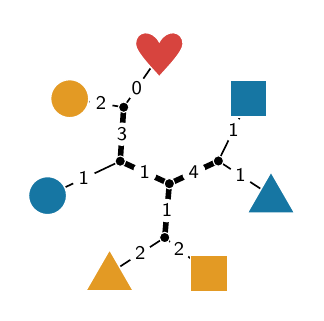
\begin{tikzpicture}[x=1.0cm,y=1.0cm,baseline=(current bounding box.center)]
\coordinate (v1) at (1.13770,0.90728);
\coordinate (v2) at (1.41868,-0.32381);
\coordinate (v3) at (-1.41868,-0.32381);
\coordinate (v4) at (0.63137,-1.31106);
\coordinate (v5) at (-0.63137,-1.31106);
\coordinate (v6) at (-1.13770,0.90728);
\coordinate (v7) at (0.00000,1.45517);
\coordinate (v8) at (0.75079,0.11610);
\coordinate (v9) at (-0.45173,0.79874);
\coordinate (v10) at (-0.49596,0.11377);
\coordinate (v11) at (0.06894,-0.85624);
\coordinate (v12) at (0.12795,-0.17238);
\draw[g2tree internal] (v8)--(v12);
\draw[g2tree internal] (v9)--(v10);
\draw[g2tree internal] (v10)--(v12);
\draw[g2tree internal] (v11)--(v12);
\draw[g2tree pendant] (v1)--(v8);
\draw[g2tree pendant] (v2)--(v8);
\draw[g2tree pendant] (v3)--(v10);
\draw[g2tree pendant] (v4)--(v11);
\draw[g2tree pendant] (v5)--(v11);
\draw[g2tree pendant] (v6)--(v9);
\draw[g2tree pendant] (v7)--(v9);
\node[g2tree weight,font={\sffamily\fontsize{7.5}{8}\selectfont}] at (0.43937,-0.02814) {4};
\node[g2tree weight,font={\sffamily\fontsize{7.5}{8}\selectfont}] at (-0.47384,0.45626) {3};
\node[g2tree weight,font={\sffamily\fontsize{7.5}{8}\selectfont}] at (-0.18400,-0.02930) {1};
\node[g2tree weight,font={\sffamily\fontsize{7.5}{8}\selectfont}] at (0.09845,-0.51431) {1};
\node[g2tree weight,font={\sffamily\fontsize{7.5}{8}\selectfont}] at (0.94424,0.51169) {1};
\node[g2tree weight,font={\sffamily\fontsize{7.5}{8}\selectfont}] at (1.03147,-0.06876) {1};
\node[g2tree weight,font={\sffamily\fontsize{7.5}{8}\selectfont}] at (-0.95732,-0.10502) {1};
\node[g2tree weight,font={\sffamily\fontsize{7.5}{8}\selectfont}] at (0.25173,-1.00406) {2};
\node[g2tree weight,font={\sffamily\fontsize{7.5}{8}\selectfont}] at (-0.24252,-1.05852) {2};
\node[g2tree weight,font={\sffamily\fontsize{7.5}{8}\selectfont}] at (-0.73973,0.84431) {2};
\node[g2tree weight,font={\sffamily\fontsize{7.5}{8}\selectfont}] at (-0.28581,1.03984) {0};
\node[g2tree vertex] at (v8) {};
\node[g2tree vertex] at (v9) {};
\node[g2tree vertex] at (v10) {};
\node[g2tree vertex] at (v11) {};
\node[g2tree vertex] at (v12) {};
\node[g2tree dark,rectangle,minimum size=4.657500000000001mm,font={\sffamily\fontsize{9}{9}\selectfont\bfseries}] at (v1) {};
\begin{scope}[shift={(v2)},scale=1.0125000000000002,transform shape]
\path[fill=g2TaxonBlue,draw=white,line width=.55pt,line join=round] (0mm,3.0mm)--(-3.0mm,-2.2mm)--(3.0mm,-2.2mm)--cycle;
\end{scope}
\node[g2tree dark,circle,minimum size=4.86mm,font={\sffamily\fontsize{9}{9}\selectfont\bfseries}] at (v3) {};
\node[g2tree light,rectangle,minimum size=4.657500000000001mm,font={\sffamily\fontsize{9}{9}\selectfont\bfseries}] at (v4) {};
\begin{scope}[shift={(v5)},scale=1.0125000000000002,transform shape]
\path[fill=g2TaxonYellow,draw=white,line width=.55pt,line join=round] (0mm,3.0mm)--(-3.0mm,-2.2mm)--(3.0mm,-2.2mm)--cycle;
\end{scope}
\node[g2tree light,circle,minimum size=4.86mm,font={\sffamily\fontsize{9}{9}\selectfont\bfseries}] at (v6) {};
\begin{scope}[shift={(v7)},scale=1.0125000000000002,transform shape]
\path[fill=g2HeartRed,draw=white,line width=.55pt]
  (0mm,-2.7mm)..controls(-.45mm,-2.1mm)and(-3.0mm,.35mm)..(-3.0mm,1.45mm)
  ..controls(-3.0mm,3.2mm)and(-.9mm,3.4mm)..(0mm,1.75mm)
  ..controls(.9mm,3.4mm)and(3.0mm,3.2mm)..(3.0mm,1.45mm)
  ..controls(3.0mm,.35mm)and(.45mm,-2.1mm)..(0mm,-2.7mm)--cycle;
\end{scope}
\end{tikzpicture}
\endgroup
\par}
\end{minipage}
 & 
\begin{minipage}[t]{\linewidth}
\noindent\textcolor{g2TreeRule}{\rule{\linewidth}{1pt}}\par
\noindent\textcolor[HTML]{000000}{\smash[b]{\textpdfrender{TextRenderingMode=FillStroke,LineWidth=.5pt}{\Large\bfseries\boldmath \oldstylenums{29}}{\large(6)}}}\par
\vskip -2.5mm
{\centering
\begingroup
\definecolor{g2TaxonBlue}{HTML}{1676A3}
\definecolor{g2TaxonYellow}{HTML}{E39A24}
\definecolor{g2HeartRed}{HTML}{D7443E}
\tikzset{
  g2tree pendant/.style={draw=black,line width=.6pt,line cap=round},
  g2tree internal/.style={draw=black,line width=2pt,line cap=round},
  g2tree vertex/.style={circle,fill=black,draw=white,line width=.4pt,inner sep=0pt,minimum size=3.8pt},
  g2tree dark/.style={fill=g2TaxonBlue,draw=white,line width=.55pt,text=white,inner sep=0pt},
  g2tree light/.style={fill=g2TaxonYellow,draw=white,line width=.55pt,text=white,inner sep=0pt},
  g2tree weight/.style={circle,fill=white,draw=none,text=black,inner sep=.15pt,minimum size=8.5pt},
  g2tree aligned pendant/.style={fill=white,text=black,inner sep=.7pt,sloped,above=1pt,font={\sffamily\fontsize{7.5}{8}\selectfont}},
  g2tree aligned internal/.style={fill=white,text=black,inner sep=1pt,sloped,above=1pt,font={\sffamily\fontsize{7.5}{8}\selectfont\bfseries}},
}
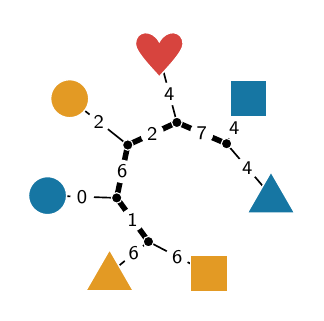
\begin{tikzpicture}[x=1.0cm,y=1.0cm,baseline=(current bounding box.center)]
\coordinate (v1) at (1.13770,0.90728);
\coordinate (v2) at (1.41868,-0.32381);
\coordinate (v3) at (-1.41868,-0.32381);
\coordinate (v4) at (0.63137,-1.31106);
\coordinate (v5) at (-0.63137,-1.31106);
\coordinate (v6) at (-1.13770,0.90728);
\coordinate (v7) at (0.00000,1.45517);
\coordinate (v8) at (0.85466,0.33590);
\coordinate (v9) at (0.22357,0.60586);
\coordinate (v10) at (-0.40001,0.31899);
\coordinate (v11) at (-0.54092,-0.35279);
\coordinate (v12) at (-0.13730,-0.90798);
\draw[g2tree internal] (v8)--(v9);
\draw[g2tree internal] (v9)--(v10);
\draw[g2tree internal] (v10)--(v11);
\draw[g2tree internal] (v11)--(v12);
\draw[g2tree pendant] (v1)--(v8);
\draw[g2tree pendant] (v2)--(v8);
\draw[g2tree pendant] (v3)--(v11);
\draw[g2tree pendant] (v4)--(v12);
\draw[g2tree pendant] (v5)--(v12);
\draw[g2tree pendant] (v6)--(v10);
\draw[g2tree pendant] (v7)--(v9);
\node[g2tree weight,font={\sffamily\fontsize{7.5}{8}\selectfont}] at (0.53912,0.47088) {7};
\node[g2tree weight,font={\sffamily\fontsize{7.5}{8}\selectfont}] at (-0.08822,0.46243) {2};
\node[g2tree weight,font={\sffamily\fontsize{7.5}{8}\selectfont}] at (-0.47046,-0.01690) {6};
\node[g2tree weight,font={\sffamily\fontsize{7.5}{8}\selectfont}] at (-0.33911,-0.63038) {1};
\node[g2tree weight,font={\sffamily\fontsize{7.5}{8}\selectfont}] at (0.95372,0.53589) {4};
\node[g2tree weight,font={\sffamily\fontsize{7.5}{8}\selectfont}] at (1.11738,0.02861) {4};
\node[g2tree weight,font={\sffamily\fontsize{7.5}{8}\selectfont}] at (-0.97980,-0.33830) {0};
\node[g2tree weight,font={\sffamily\fontsize{7.5}{8}\selectfont}] at (0.22782,-1.09944) {6};
\node[g2tree weight,font={\sffamily\fontsize{7.5}{8}\selectfont}] at (-0.32258,-1.05913) {6};
\node[g2tree weight,font={\sffamily\fontsize{7.5}{8}\selectfont}] at (-0.76885,0.61314) {2};
\node[g2tree weight,font={\sffamily\fontsize{7.5}{8}\selectfont}] at (0.12835,0.96761) {4};
\node[g2tree vertex] at (v8) {};
\node[g2tree vertex] at (v9) {};
\node[g2tree vertex] at (v10) {};
\node[g2tree vertex] at (v11) {};
\node[g2tree vertex] at (v12) {};
\node[g2tree dark,rectangle,minimum size=4.657500000000001mm,font={\sffamily\fontsize{9}{9}\selectfont\bfseries}] at (v1) {};
\begin{scope}[shift={(v2)},scale=1.0125000000000002,transform shape]
\path[fill=g2TaxonBlue,draw=white,line width=.55pt,line join=round] (0mm,3.0mm)--(-3.0mm,-2.2mm)--(3.0mm,-2.2mm)--cycle;
\end{scope}
\node[g2tree dark,circle,minimum size=4.86mm,font={\sffamily\fontsize{9}{9}\selectfont\bfseries}] at (v3) {};
\node[g2tree light,rectangle,minimum size=4.657500000000001mm,font={\sffamily\fontsize{9}{9}\selectfont\bfseries}] at (v4) {};
\begin{scope}[shift={(v5)},scale=1.0125000000000002,transform shape]
\path[fill=g2TaxonYellow,draw=white,line width=.55pt,line join=round] (0mm,3.0mm)--(-3.0mm,-2.2mm)--(3.0mm,-2.2mm)--cycle;
\end{scope}
\node[g2tree light,circle,minimum size=4.86mm,font={\sffamily\fontsize{9}{9}\selectfont\bfseries}] at (v6) {};
\begin{scope}[shift={(v7)},scale=1.0125000000000002,transform shape]
\path[fill=g2HeartRed,draw=white,line width=.55pt]
  (0mm,-2.7mm)..controls(-.45mm,-2.1mm)and(-3.0mm,.35mm)..(-3.0mm,1.45mm)
  ..controls(-3.0mm,3.2mm)and(-.9mm,3.4mm)..(0mm,1.75mm)
  ..controls(.9mm,3.4mm)and(3.0mm,3.2mm)..(3.0mm,1.45mm)
  ..controls(3.0mm,.35mm)and(.45mm,-2.1mm)..(0mm,-2.7mm)--cycle;
\end{scope}
\end{tikzpicture}
\endgroup
\par}
\end{minipage}
\\\noalign{\vskip 0.22cm}
\begin{minipage}[t]{\linewidth}
\noindent\textcolor{g2TreeRule}{\rule{\linewidth}{1pt}}\par
\noindent\textcolor[HTML]{000000}{\smash[b]{\textpdfrender{TextRenderingMode=FillStroke,LineWidth=.5pt}{\Large\bfseries\boldmath \oldstylenums{30}}{\large(3)}}}\hfill\smash[b]{\tikz[baseline=0pt]\draw[g2TreeRule,line width=1pt] (0,0) rectangle (2.6mm,2.6mm);}\par
\vskip -2.5mm
{\centering
\begingroup
\definecolor{g2TaxonBlue}{HTML}{1676A3}
\definecolor{g2TaxonYellow}{HTML}{E39A24}
\definecolor{g2HeartRed}{HTML}{D7443E}
\tikzset{
  g2tree pendant/.style={draw=black,line width=.6pt,line cap=round},
  g2tree internal/.style={draw=black,line width=2pt,line cap=round},
  g2tree vertex/.style={circle,fill=black,draw=white,line width=.4pt,inner sep=0pt,minimum size=3.8pt},
  g2tree dark/.style={fill=g2TaxonBlue,draw=white,line width=.55pt,text=white,inner sep=0pt},
  g2tree light/.style={fill=g2TaxonYellow,draw=white,line width=.55pt,text=white,inner sep=0pt},
  g2tree weight/.style={circle,fill=white,draw=none,text=black,inner sep=.15pt,minimum size=8.5pt},
  g2tree aligned pendant/.style={fill=white,text=black,inner sep=.7pt,sloped,above=1pt,font={\sffamily\fontsize{7.5}{8}\selectfont}},
  g2tree aligned internal/.style={fill=white,text=black,inner sep=1pt,sloped,above=1pt,font={\sffamily\fontsize{7.5}{8}\selectfont\bfseries}},
}
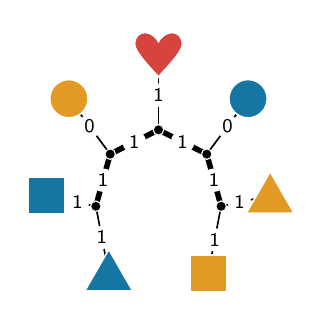
\begin{tikzpicture}[x=1.0cm,y=1.0cm,baseline=(current bounding box.center)]
\coordinate (v1) at (-1.41868,-0.32381);
\coordinate (v2) at (-0.63137,-1.31106);
\coordinate (v3) at (1.13770,0.90728);
\coordinate (v4) at (0.63137,-1.31106);
\coordinate (v5) at (1.41868,-0.32381);
\coordinate (v6) at (-1.13770,0.90728);
\coordinate (v7) at (0.00000,1.45517);
\coordinate (v8) at (-0.79549,-0.45877);
\coordinate (v9) at (0.79549,-0.45877);
\coordinate (v10) at (0.61308,0.20295);
\coordinate (v11) at (-0.61308,0.20295);
\coordinate (v12) at (-0.00000,0.51163);
\draw[g2tree internal] (v8)--(v11);
\draw[g2tree internal] (v9)--(v10);
\draw[g2tree internal] (v10)--(v12);
\draw[g2tree internal] (v11)--(v12);
\draw[g2tree pendant] (v1)--(v8);
\draw[g2tree pendant] (v2)--(v8);
\draw[g2tree pendant] (v3)--(v10);
\draw[g2tree pendant] (v4)--(v9);
\draw[g2tree pendant] (v5)--(v9);
\draw[g2tree pendant] (v6)--(v11);
\draw[g2tree pendant] (v7)--(v12);
\node[g2tree weight,font={\sffamily\fontsize{7.5}{8}\selectfont}] at (-0.70428,-0.12791) {1};
\node[g2tree weight,font={\sffamily\fontsize{7.5}{8}\selectfont}] at (0.70428,-0.12791) {1};
\node[g2tree weight,font={\sffamily\fontsize{7.5}{8}\selectfont}] at (0.30654,0.35729) {1};
\node[g2tree weight,font={\sffamily\fontsize{7.5}{8}\selectfont}] at (-0.30654,0.35729) {1};
\node[g2tree weight,font={\sffamily\fontsize{7.5}{8}\selectfont}] at (-1.02919,-0.40816) {1};
\node[g2tree weight,font={\sffamily\fontsize{7.5}{8}\selectfont}] at (-0.71905,-0.85576) {1};
\node[g2tree weight,font={\sffamily\fontsize{7.5}{8}\selectfont}] at (0.87539,0.55512) {0};
\node[g2tree weight,font={\sffamily\fontsize{7.5}{8}\selectfont}] at (0.71343,-0.88491) {1};
\node[g2tree weight,font={\sffamily\fontsize{7.5}{8}\selectfont}] at (1.02919,-0.40816) {1};
\node[g2tree weight,font={\sffamily\fontsize{7.5}{8}\selectfont}] at (-0.87539,0.55512) {0};
\node[g2tree weight,font={\sffamily\fontsize{7.5}{8}\selectfont}] at (0.00000,0.95100) {1};
\node[g2tree vertex] at (v8) {};
\node[g2tree vertex] at (v9) {};
\node[g2tree vertex] at (v10) {};
\node[g2tree vertex] at (v11) {};
\node[g2tree vertex] at (v12) {};
\node[g2tree dark,rectangle,minimum size=4.657500000000001mm,font={\sffamily\fontsize{9}{9}\selectfont\bfseries}] at (v1) {};
\begin{scope}[shift={(v2)},scale=1.0125000000000002,transform shape]
\path[fill=g2TaxonBlue,draw=white,line width=.55pt,line join=round] (0mm,3.0mm)--(-3.0mm,-2.2mm)--(3.0mm,-2.2mm)--cycle;
\end{scope}
\node[g2tree dark,circle,minimum size=4.86mm,font={\sffamily\fontsize{9}{9}\selectfont\bfseries}] at (v3) {};
\node[g2tree light,rectangle,minimum size=4.657500000000001mm,font={\sffamily\fontsize{9}{9}\selectfont\bfseries}] at (v4) {};
\begin{scope}[shift={(v5)},scale=1.0125000000000002,transform shape]
\path[fill=g2TaxonYellow,draw=white,line width=.55pt,line join=round] (0mm,3.0mm)--(-3.0mm,-2.2mm)--(3.0mm,-2.2mm)--cycle;
\end{scope}
\node[g2tree light,circle,minimum size=4.86mm,font={\sffamily\fontsize{9}{9}\selectfont\bfseries}] at (v6) {};
\begin{scope}[shift={(v7)},scale=1.0125000000000002,transform shape]
\path[fill=g2HeartRed,draw=white,line width=.55pt]
  (0mm,-2.7mm)..controls(-.45mm,-2.1mm)and(-3.0mm,.35mm)..(-3.0mm,1.45mm)
  ..controls(-3.0mm,3.2mm)and(-.9mm,3.4mm)..(0mm,1.75mm)
  ..controls(.9mm,3.4mm)and(3.0mm,3.2mm)..(3.0mm,1.45mm)
  ..controls(3.0mm,.35mm)and(.45mm,-2.1mm)..(0mm,-2.7mm)--cycle;
\end{scope}
\end{tikzpicture}
\endgroup
\par}
\end{minipage}
 & 
\multicolumn{1}{p{4.7cm}@{\hspace{\dimexpr0.11cm-1pt/2\relax}{\color{g2TreeRule}\vrule width 1pt height 1pt}\hspace{\dimexpr0.11cm-1pt/2\relax}}}{%
\begin{minipage}[t]{\linewidth}
\noindent\textcolor{g2TreeRule}{\rule{\linewidth}{1pt}}\par
\noindent\textcolor[HTML]{000000}{\smash[b]{\textpdfrender{TextRenderingMode=FillStroke,LineWidth=.5pt}{\Large\bfseries\boldmath \oldstylenums{31}}{\large(12)}}}\par
\vskip -2.5mm
{\centering
\begingroup
\definecolor{g2TaxonBlue}{HTML}{1676A3}
\definecolor{g2TaxonYellow}{HTML}{E39A24}
\definecolor{g2HeartRed}{HTML}{D7443E}
\tikzset{
  g2tree pendant/.style={draw=black,line width=.6pt,line cap=round},
  g2tree internal/.style={draw=black,line width=2pt,line cap=round},
  g2tree vertex/.style={circle,fill=black,draw=white,line width=.4pt,inner sep=0pt,minimum size=3.8pt},
  g2tree dark/.style={fill=g2TaxonBlue,draw=white,line width=.55pt,text=white,inner sep=0pt},
  g2tree light/.style={fill=g2TaxonYellow,draw=white,line width=.55pt,text=white,inner sep=0pt},
  g2tree weight/.style={circle,fill=white,draw=none,text=black,inner sep=.15pt,minimum size=8.5pt},
  g2tree aligned pendant/.style={fill=white,text=black,inner sep=.7pt,sloped,above=1pt,font={\sffamily\fontsize{7.5}{8}\selectfont}},
  g2tree aligned internal/.style={fill=white,text=black,inner sep=1pt,sloped,above=1pt,font={\sffamily\fontsize{7.5}{8}\selectfont\bfseries}},
}
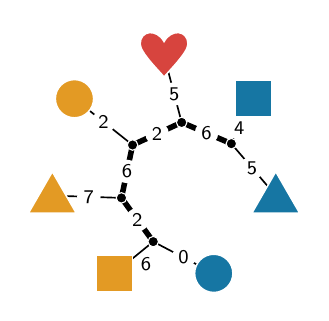
\begin{tikzpicture}[x=1.0cm,y=1.0cm,baseline=(current bounding box.center)]
\coordinate (v1) at (1.13770,0.90728);
\coordinate (v2) at (1.41868,-0.32381);
\coordinate (v3) at (0.63137,-1.31106);
\coordinate (v4) at (-0.63137,-1.31106);
\coordinate (v5) at (-1.41868,-0.32381);
\coordinate (v6) at (-1.13770,0.90728);
\coordinate (v7) at (0.00000,1.45517);
\coordinate (v8) at (0.85466,0.33590);
\coordinate (v9) at (-0.13730,-0.90798);
\coordinate (v10) at (-0.54092,-0.35279);
\coordinate (v11) at (-0.40001,0.31899);
\coordinate (v12) at (0.22357,0.60586);
\draw[g2tree internal] (v8)--(v12);
\draw[g2tree internal] (v9)--(v10);
\draw[g2tree internal] (v10)--(v11);
\draw[g2tree internal] (v11)--(v12);
\draw[g2tree pendant] (v1)--(v8);
\draw[g2tree pendant] (v2)--(v8);
\draw[g2tree pendant] (v3)--(v9);
\draw[g2tree pendant] (v4)--(v9);
\draw[g2tree pendant] (v5)--(v10);
\draw[g2tree pendant] (v6)--(v11);
\draw[g2tree pendant] (v7)--(v12);
\node[g2tree weight,font={\sffamily\fontsize{7.5}{8}\selectfont}] at (0.53912,0.47088) {6};
\node[g2tree weight,font={\sffamily\fontsize{7.5}{8}\selectfont}] at (-0.33911,-0.63038) {2};
\node[g2tree weight,font={\sffamily\fontsize{7.5}{8}\selectfont}] at (-0.47046,-0.01690) {6};
\node[g2tree weight,font={\sffamily\fontsize{7.5}{8}\selectfont}] at (-0.08822,0.46243) {2};
\node[g2tree weight,font={\sffamily\fontsize{7.5}{8}\selectfont}] at (0.95372,0.53589) {4};
\node[g2tree weight,font={\sffamily\fontsize{7.5}{8}\selectfont}] at (1.11738,0.02861) {5};
\node[g2tree weight,font={\sffamily\fontsize{7.5}{8}\selectfont}] at (0.24704,-1.10952) {0};
\node[g2tree weight,font={\sffamily\fontsize{7.5}{8}\selectfont}] at (-0.22940,-1.19856) {6};
\node[g2tree weight,font={\sffamily\fontsize{7.5}{8}\selectfont}] at (-0.95527,-0.33911) {7};
\node[g2tree weight,font={\sffamily\fontsize{7.5}{8}\selectfont}] at (-0.76885,0.61314) {2};
\node[g2tree weight,font={\sffamily\fontsize{7.5}{8}\selectfont}] at (0.12835,0.96761) {5};
\node[g2tree vertex] at (v8) {};
\node[g2tree vertex] at (v9) {};
\node[g2tree vertex] at (v10) {};
\node[g2tree vertex] at (v11) {};
\node[g2tree vertex] at (v12) {};
\node[g2tree dark,rectangle,minimum size=4.657500000000001mm,font={\sffamily\fontsize{9}{9}\selectfont\bfseries}] at (v1) {};
\begin{scope}[shift={(v2)},scale=1.0125000000000002,transform shape]
\path[fill=g2TaxonBlue,draw=white,line width=.55pt,line join=round] (0mm,3.0mm)--(-3.0mm,-2.2mm)--(3.0mm,-2.2mm)--cycle;
\end{scope}
\node[g2tree dark,circle,minimum size=4.86mm,font={\sffamily\fontsize{9}{9}\selectfont\bfseries}] at (v3) {};
\node[g2tree light,rectangle,minimum size=4.657500000000001mm,font={\sffamily\fontsize{9}{9}\selectfont\bfseries}] at (v4) {};
\begin{scope}[shift={(v5)},scale=1.0125000000000002,transform shape]
\path[fill=g2TaxonYellow,draw=white,line width=.55pt,line join=round] (0mm,3.0mm)--(-3.0mm,-2.2mm)--(3.0mm,-2.2mm)--cycle;
\end{scope}
\node[g2tree light,circle,minimum size=4.86mm,font={\sffamily\fontsize{9}{9}\selectfont\bfseries}] at (v6) {};
\begin{scope}[shift={(v7)},scale=1.0125000000000002,transform shape]
\path[fill=g2HeartRed,draw=white,line width=.55pt]
  (0mm,-2.7mm)..controls(-.45mm,-2.1mm)and(-3.0mm,.35mm)..(-3.0mm,1.45mm)
  ..controls(-3.0mm,3.2mm)and(-.9mm,3.4mm)..(0mm,1.75mm)
  ..controls(.9mm,3.4mm)and(3.0mm,3.2mm)..(3.0mm,1.45mm)
  ..controls(3.0mm,.35mm)and(.45mm,-2.1mm)..(0mm,-2.7mm)--cycle;
\end{scope}
\end{tikzpicture}
\endgroup
\par}
\end{minipage}}
 & 
\begin{minipage}[t]{\linewidth}
\noindent\textcolor{g2TreeRule}{\rule{\linewidth}{1pt}}\par
\noindent\textcolor[HTML]{000000}{\smash[b]{\textpdfrender{TextRenderingMode=FillStroke,LineWidth=.5pt}{\Large\bfseries\boldmath \oldstylenums{32}}{\large(6)}}}\par
\vskip -2.5mm
{\centering
\begingroup
\definecolor{g2TaxonBlue}{HTML}{1676A3}
\definecolor{g2TaxonYellow}{HTML}{E39A24}
\definecolor{g2HeartRed}{HTML}{D7443E}
\tikzset{
  g2tree pendant/.style={draw=black,line width=.6pt,line cap=round},
  g2tree internal/.style={draw=black,line width=2pt,line cap=round},
  g2tree vertex/.style={circle,fill=black,draw=white,line width=.4pt,inner sep=0pt,minimum size=3.8pt},
  g2tree dark/.style={fill=g2TaxonBlue,draw=white,line width=.55pt,text=white,inner sep=0pt},
  g2tree light/.style={fill=g2TaxonYellow,draw=white,line width=.55pt,text=white,inner sep=0pt},
  g2tree weight/.style={circle,fill=white,draw=none,text=black,inner sep=.15pt,minimum size=8.5pt},
  g2tree aligned pendant/.style={fill=white,text=black,inner sep=.7pt,sloped,above=1pt,font={\sffamily\fontsize{7.5}{8}\selectfont}},
  g2tree aligned internal/.style={fill=white,text=black,inner sep=1pt,sloped,above=1pt,font={\sffamily\fontsize{7.5}{8}\selectfont\bfseries}},
}
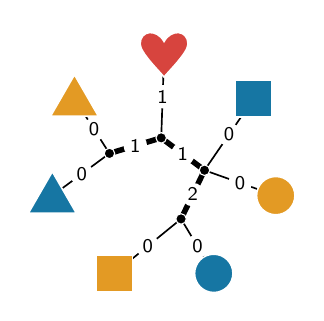
\begin{tikzpicture}[x=1.0cm,y=1.0cm,baseline=(current bounding box.center)]
\coordinate (v1) at (1.13770,0.90728);
\coordinate (v2) at (-1.41868,-0.32381);
\coordinate (v3) at (0.63137,-1.31106);
\coordinate (v4) at (-0.63137,-1.31106);
\coordinate (v5) at (-1.13770,0.90728);
\coordinate (v6) at (1.41868,-0.32381);
\coordinate (v7) at (0.00000,1.45517);
\coordinate (v8) at (0.21583,-0.61994);
\coordinate (v9) at (-0.69348,0.21207);
\coordinate (v10) at (-0.03607,0.40941);
\coordinate (v11) at (0.51372,-0.00154);
\draw[g2tree internal] (v8)--(v11);
\draw[g2tree internal] (v9)--(v10);
\draw[g2tree internal] (v10)--(v11);
\draw[g2tree pendant] (v1)--(v11);
\draw[g2tree pendant] (v2)--(v9);
\draw[g2tree pendant] (v3)--(v8);
\draw[g2tree pendant] (v4)--(v8);
\draw[g2tree pendant] (v5)--(v9);
\draw[g2tree pendant] (v6)--(v11);
\draw[g2tree pendant] (v7)--(v10);
\node[g2tree weight,font={\sffamily\fontsize{7.5}{8}\selectfont}] at (0.36478,-0.31074) {2};
\node[g2tree weight,font={\sffamily\fontsize{7.5}{8}\selectfont}] at (-0.36478,0.31074) {1};
\node[g2tree weight,font={\sffamily\fontsize{7.5}{8}\selectfont}] at (0.23882,0.20393) {1};
\node[g2tree weight,font={\sffamily\fontsize{7.5}{8}\selectfont}] at (0.82571,0.45287) {0};
\node[g2tree weight,font={\sffamily\fontsize{7.5}{8}\selectfont}] at (-1.04578,-0.04825) {0};
\node[g2tree weight,font={\sffamily\fontsize{7.5}{8}\selectfont}] at (0.42360,-0.96550) {0};
\node[g2tree weight,font={\sffamily\fontsize{7.5}{8}\selectfont}] at (-0.20777,-0.96550) {0};
\node[g2tree weight,font={\sffamily\fontsize{7.5}{8}\selectfont}] at (-0.88805,0.51657) {0};
\node[g2tree weight,font={\sffamily\fontsize{7.5}{8}\selectfont}] at (0.96620,-0.16267) {0};
\node[g2tree weight,font={\sffamily\fontsize{7.5}{8}\selectfont}] at (-0.01803,0.93229) {1};
\node[g2tree vertex] at (v8) {};
\node[g2tree vertex] at (v9) {};
\node[g2tree vertex] at (v10) {};
\node[g2tree vertex] at (v11) {};
\node[g2tree dark,rectangle,minimum size=4.657500000000001mm,font={\sffamily\fontsize{9}{9}\selectfont\bfseries}] at (v1) {};
\begin{scope}[shift={(v2)},scale=1.0125000000000002,transform shape]
\path[fill=g2TaxonBlue,draw=white,line width=.55pt,line join=round] (0mm,3.0mm)--(-3.0mm,-2.2mm)--(3.0mm,-2.2mm)--cycle;
\end{scope}
\node[g2tree dark,circle,minimum size=4.86mm,font={\sffamily\fontsize{9}{9}\selectfont\bfseries}] at (v3) {};
\node[g2tree light,rectangle,minimum size=4.657500000000001mm,font={\sffamily\fontsize{9}{9}\selectfont\bfseries}] at (v4) {};
\begin{scope}[shift={(v5)},scale=1.0125000000000002,transform shape]
\path[fill=g2TaxonYellow,draw=white,line width=.55pt,line join=round] (0mm,3.0mm)--(-3.0mm,-2.2mm)--(3.0mm,-2.2mm)--cycle;
\end{scope}
\node[g2tree light,circle,minimum size=4.86mm,font={\sffamily\fontsize{9}{9}\selectfont\bfseries}] at (v6) {};
\begin{scope}[shift={(v7)},scale=1.0125000000000002,transform shape]
\path[fill=g2HeartRed,draw=white,line width=.55pt]
  (0mm,-2.7mm)..controls(-.45mm,-2.1mm)and(-3.0mm,.35mm)..(-3.0mm,1.45mm)
  ..controls(-3.0mm,3.2mm)and(-.9mm,3.4mm)..(0mm,1.75mm)
  ..controls(.9mm,3.4mm)and(3.0mm,3.2mm)..(3.0mm,1.45mm)
  ..controls(3.0mm,.35mm)and(.45mm,-2.1mm)..(0mm,-2.7mm)--cycle;
\end{scope}
\end{tikzpicture}
\endgroup
\par}
\vskip 0pt plus 1filll
\noindent\rlap{char\ \(\neq 2\)}\par
\end{minipage}
\\\noalign{\vskip 0.22cm}
\begin{minipage}[t]{\linewidth}
\noindent\textcolor{g2TreeRule}{\rule{\linewidth}{1pt}}\par
\noindent\textcolor[HTML]{000000}{\smash[b]{\textpdfrender{TextRenderingMode=FillStroke,LineWidth=.5pt}{\Large\bfseries\boldmath \oldstylenums{33}}{\large(3)}}}\par
\vskip -2.5mm
{\centering
\begingroup
\definecolor{g2TaxonBlue}{HTML}{1676A3}
\definecolor{g2TaxonYellow}{HTML}{E39A24}
\definecolor{g2HeartRed}{HTML}{D7443E}
\tikzset{
  g2tree pendant/.style={draw=black,line width=.6pt,line cap=round},
  g2tree internal/.style={draw=black,line width=2pt,line cap=round},
  g2tree vertex/.style={circle,fill=black,draw=white,line width=.4pt,inner sep=0pt,minimum size=3.8pt},
  g2tree dark/.style={fill=g2TaxonBlue,draw=white,line width=.55pt,text=white,inner sep=0pt},
  g2tree light/.style={fill=g2TaxonYellow,draw=white,line width=.55pt,text=white,inner sep=0pt},
  g2tree weight/.style={circle,fill=white,draw=none,text=black,inner sep=.15pt,minimum size=8.5pt},
  g2tree aligned pendant/.style={fill=white,text=black,inner sep=.7pt,sloped,above=1pt,font={\sffamily\fontsize{7.5}{8}\selectfont}},
  g2tree aligned internal/.style={fill=white,text=black,inner sep=1pt,sloped,above=1pt,font={\sffamily\fontsize{7.5}{8}\selectfont\bfseries}},
}
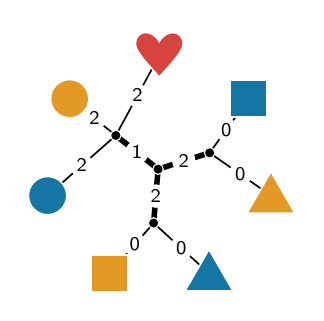
\begin{tikzpicture}[x=1.0cm,y=1.0cm,baseline=(current bounding box.center)]
\coordinate (v1) at (1.13770,0.90728);
\coordinate (v2) at (0.63137,-1.31106);
\coordinate (v3) at (-1.41868,-0.32381);
\coordinate (v4) at (-0.63137,-1.31106);
\coordinate (v5) at (1.41868,-0.32381);
\coordinate (v6) at (-1.13770,0.90728);
\coordinate (v7) at (0.00000,1.45517);
\coordinate (v8) at (0.63906,0.21978);
\coordinate (v9) at (-0.07206,-0.67194);
\coordinate (v10) at (-0.01517,0.01210);
\coordinate (v11) at (-0.55182,0.44006);
\draw[g2tree internal] (v8)--(v10);
\draw[g2tree internal] (v9)--(v10);
\draw[g2tree internal] (v10)--(v11);
\draw[g2tree pendant] (v1)--(v8);
\draw[g2tree pendant] (v2)--(v9);
\draw[g2tree pendant] (v3)--(v11);
\draw[g2tree pendant] (v4)--(v9);
\draw[g2tree pendant] (v5)--(v8);
\draw[g2tree pendant] (v6)--(v11);
\draw[g2tree pendant] (v7)--(v11);
\node[g2tree weight,font={\sffamily\fontsize{7.5}{8}\selectfont}] at (0.31194,0.11594) {2};
\node[g2tree weight,font={\sffamily\fontsize{7.5}{8}\selectfont}] at (-0.04362,-0.32992) {2};
\node[g2tree weight,font={\sffamily\fontsize{7.5}{8}\selectfont}] at (-0.28350,0.22608) {1};
\node[g2tree weight,font={\sffamily\fontsize{7.5}{8}\selectfont}] at (0.85098,0.51197) {0};
\node[g2tree weight,font={\sffamily\fontsize{7.5}{8}\selectfont}] at (0.27966,-0.99150) {0};
\node[g2tree weight,font={\sffamily\fontsize{7.5}{8}\selectfont}] at (-0.98525,0.05813) {2};
\node[g2tree weight,font={\sffamily\fontsize{7.5}{8}\selectfont}] at (-0.30977,-0.94357) {0};
\node[g2tree weight,font={\sffamily\fontsize{7.5}{8}\selectfont}] at (1.02887,-0.05201) {0};
\node[g2tree weight,font={\sffamily\fontsize{7.5}{8}\selectfont}] at (-0.82269,0.65607) {2};
\node[g2tree weight,font={\sffamily\fontsize{7.5}{8}\selectfont}] at (-0.27591,0.94762) {2};
\node[g2tree vertex] at (v8) {};
\node[g2tree vertex] at (v9) {};
\node[g2tree vertex] at (v10) {};
\node[g2tree vertex] at (v11) {};
\node[g2tree dark,rectangle,minimum size=4.657500000000001mm,font={\sffamily\fontsize{9}{9}\selectfont\bfseries}] at (v1) {};
\begin{scope}[shift={(v2)},scale=1.0125000000000002,transform shape]
\path[fill=g2TaxonBlue,draw=white,line width=.55pt,line join=round] (0mm,3.0mm)--(-3.0mm,-2.2mm)--(3.0mm,-2.2mm)--cycle;
\end{scope}
\node[g2tree dark,circle,minimum size=4.86mm,font={\sffamily\fontsize{9}{9}\selectfont\bfseries}] at (v3) {};
\node[g2tree light,rectangle,minimum size=4.657500000000001mm,font={\sffamily\fontsize{9}{9}\selectfont\bfseries}] at (v4) {};
\begin{scope}[shift={(v5)},scale=1.0125000000000002,transform shape]
\path[fill=g2TaxonYellow,draw=white,line width=.55pt,line join=round] (0mm,3.0mm)--(-3.0mm,-2.2mm)--(3.0mm,-2.2mm)--cycle;
\end{scope}
\node[g2tree light,circle,minimum size=4.86mm,font={\sffamily\fontsize{9}{9}\selectfont\bfseries}] at (v6) {};
\begin{scope}[shift={(v7)},scale=1.0125000000000002,transform shape]
\path[fill=g2HeartRed,draw=white,line width=.55pt]
  (0mm,-2.7mm)..controls(-.45mm,-2.1mm)and(-3.0mm,.35mm)..(-3.0mm,1.45mm)
  ..controls(-3.0mm,3.2mm)and(-.9mm,3.4mm)..(0mm,1.75mm)
  ..controls(.9mm,3.4mm)and(3.0mm,3.2mm)..(3.0mm,1.45mm)
  ..controls(3.0mm,.35mm)and(.45mm,-2.1mm)..(0mm,-2.7mm)--cycle;
\end{scope}
\end{tikzpicture}
\endgroup
\par}
\vskip 0pt plus 1filll
\noindent\rlap{char\ \(\neq 2\)}\par
\end{minipage}
 & 
\multicolumn{1}{p{4.7cm}@{\hspace{\dimexpr0.11cm-1pt/2\relax}{\color{g2TreeRule}\vrule width 1pt height 1pt}\hspace{\dimexpr0.11cm-1pt/2\relax}}}{%
\begin{minipage}[t]{\linewidth}
\noindent\textcolor{g2TreeRule}{\rule{\linewidth}{1pt}}\par
\noindent\textcolor[HTML]{000000}{\smash[b]{\textpdfrender{TextRenderingMode=FillStroke,LineWidth=.5pt}{\Large\bfseries\boldmath \oldstylenums{34}}{\large(3)}}}\par
\vskip -2.5mm
{\centering
\begingroup
\definecolor{g2TaxonBlue}{HTML}{1676A3}
\definecolor{g2TaxonYellow}{HTML}{E39A24}
\definecolor{g2HeartRed}{HTML}{D7443E}
\tikzset{
  g2tree pendant/.style={draw=black,line width=.6pt,line cap=round},
  g2tree internal/.style={draw=black,line width=2pt,line cap=round},
  g2tree vertex/.style={circle,fill=black,draw=white,line width=.4pt,inner sep=0pt,minimum size=3.8pt},
  g2tree dark/.style={fill=g2TaxonBlue,draw=white,line width=.55pt,text=white,inner sep=0pt},
  g2tree light/.style={fill=g2TaxonYellow,draw=white,line width=.55pt,text=white,inner sep=0pt},
  g2tree weight/.style={circle,fill=white,draw=none,text=black,inner sep=.15pt,minimum size=8.5pt},
  g2tree aligned pendant/.style={fill=white,text=black,inner sep=.7pt,sloped,above=1pt,font={\sffamily\fontsize{7.5}{8}\selectfont}},
  g2tree aligned internal/.style={fill=white,text=black,inner sep=1pt,sloped,above=1pt,font={\sffamily\fontsize{7.5}{8}\selectfont\bfseries}},
}
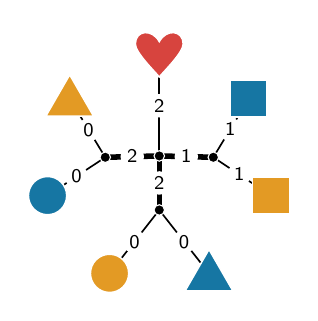
\begin{tikzpicture}[x=1.0cm,y=1.0cm,baseline=(current bounding box.center)]
\coordinate (v1) at (1.13770,0.90728);
\coordinate (v2) at (0.63137,-1.31106);
\coordinate (v3) at (-1.41868,-0.32381);
\coordinate (v4) at (1.41868,-0.32381);
\coordinate (v5) at (-1.13770,0.90728);
\coordinate (v6) at (-0.63137,-1.31106);
\coordinate (v7) at (0.00000,1.45517);
\coordinate (v8) at (0.00000,-0.50631);
\coordinate (v9) at (-0.68619,0.16311);
\coordinate (v10) at (0.68619,0.16311);
\coordinate (v11) at (0.00000,0.18009);
\draw[g2tree internal] (v8)--(v11);
\draw[g2tree internal] (v9)--(v11);
\draw[g2tree internal] (v10)--(v11);
\draw[g2tree pendant] (v1)--(v10);
\draw[g2tree pendant] (v2)--(v8);
\draw[g2tree pendant] (v3)--(v9);
\draw[g2tree pendant] (v4)--(v10);
\draw[g2tree pendant] (v5)--(v9);
\draw[g2tree pendant] (v6)--(v8);
\draw[g2tree pendant] (v7)--(v11);
\node[g2tree weight,font={\sffamily\fontsize{7.5}{8}\selectfont}] at (0.00000,-0.16311) {2};
\node[g2tree weight,font={\sffamily\fontsize{7.5}{8}\selectfont}] at (-0.34309,0.17160) {2};
\node[g2tree weight,font={\sffamily\fontsize{7.5}{8}\selectfont}] at (0.34309,0.17160) {1};
\node[g2tree weight,font={\sffamily\fontsize{7.5}{8}\selectfont}] at (0.90066,0.51659) {1};
\node[g2tree weight,font={\sffamily\fontsize{7.5}{8}\selectfont}] at (0.31569,-0.90869) {0};
\node[g2tree weight,font={\sffamily\fontsize{7.5}{8}\selectfont}] at (-1.05244,-0.08035) {0};
\node[g2tree weight,font={\sffamily\fontsize{7.5}{8}\selectfont}] at (1.01581,-0.05600) {1};
\node[g2tree weight,font={\sffamily\fontsize{7.5}{8}\selectfont}] at (-0.89719,0.51087) {0};
\node[g2tree weight,font={\sffamily\fontsize{7.5}{8}\selectfont}] at (-0.31569,-0.90869) {0};
\node[g2tree weight,font={\sffamily\fontsize{7.5}{8}\selectfont}] at (0.00000,0.81763) {2};
\node[g2tree vertex] at (v8) {};
\node[g2tree vertex] at (v9) {};
\node[g2tree vertex] at (v10) {};
\node[g2tree vertex] at (v11) {};
\node[g2tree dark,rectangle,minimum size=4.657500000000001mm,font={\sffamily\fontsize{9}{9}\selectfont\bfseries}] at (v1) {};
\begin{scope}[shift={(v2)},scale=1.0125000000000002,transform shape]
\path[fill=g2TaxonBlue,draw=white,line width=.55pt,line join=round] (0mm,3.0mm)--(-3.0mm,-2.2mm)--(3.0mm,-2.2mm)--cycle;
\end{scope}
\node[g2tree dark,circle,minimum size=4.86mm,font={\sffamily\fontsize{9}{9}\selectfont\bfseries}] at (v3) {};
\node[g2tree light,rectangle,minimum size=4.657500000000001mm,font={\sffamily\fontsize{9}{9}\selectfont\bfseries}] at (v4) {};
\begin{scope}[shift={(v5)},scale=1.0125000000000002,transform shape]
\path[fill=g2TaxonYellow,draw=white,line width=.55pt,line join=round] (0mm,3.0mm)--(-3.0mm,-2.2mm)--(3.0mm,-2.2mm)--cycle;
\end{scope}
\node[g2tree light,circle,minimum size=4.86mm,font={\sffamily\fontsize{9}{9}\selectfont\bfseries}] at (v6) {};
\begin{scope}[shift={(v7)},scale=1.0125000000000002,transform shape]
\path[fill=g2HeartRed,draw=white,line width=.55pt]
  (0mm,-2.7mm)..controls(-.45mm,-2.1mm)and(-3.0mm,.35mm)..(-3.0mm,1.45mm)
  ..controls(-3.0mm,3.2mm)and(-.9mm,3.4mm)..(0mm,1.75mm)
  ..controls(.9mm,3.4mm)and(3.0mm,3.2mm)..(3.0mm,1.45mm)
  ..controls(3.0mm,.35mm)and(.45mm,-2.1mm)..(0mm,-2.7mm)--cycle;
\end{scope}
\end{tikzpicture}
\endgroup
\par}
\vskip 0pt plus 1filll
\noindent\rlap{char\ \(\neq 2\)}\par
\end{minipage}}
 & 
\begin{minipage}[t]{\linewidth}
\noindent\textcolor{g2TreeRule}{\rule{\linewidth}{1pt}}\par
\noindent\textcolor[HTML]{000000}{\smash[b]{\textpdfrender{TextRenderingMode=FillStroke,LineWidth=.5pt}{\Large\bfseries\boldmath \oldstylenums{35}}{\large(6)}}}\par
\vskip -2.5mm
{\centering
\begingroup
\definecolor{g2TaxonBlue}{HTML}{1676A3}
\definecolor{g2TaxonYellow}{HTML}{E39A24}
\definecolor{g2HeartRed}{HTML}{D7443E}
\tikzset{
  g2tree pendant/.style={draw=black,line width=.6pt,line cap=round},
  g2tree internal/.style={draw=black,line width=2pt,line cap=round},
  g2tree vertex/.style={circle,fill=black,draw=white,line width=.4pt,inner sep=0pt,minimum size=3.8pt},
  g2tree dark/.style={fill=g2TaxonBlue,draw=white,line width=.55pt,text=white,inner sep=0pt},
  g2tree light/.style={fill=g2TaxonYellow,draw=white,line width=.55pt,text=white,inner sep=0pt},
  g2tree weight/.style={circle,fill=white,draw=none,text=black,inner sep=.15pt,minimum size=8.5pt},
  g2tree aligned pendant/.style={fill=white,text=black,inner sep=.7pt,sloped,above=1pt,font={\sffamily\fontsize{7.5}{8}\selectfont}},
  g2tree aligned internal/.style={fill=white,text=black,inner sep=1pt,sloped,above=1pt,font={\sffamily\fontsize{7.5}{8}\selectfont\bfseries}},
}
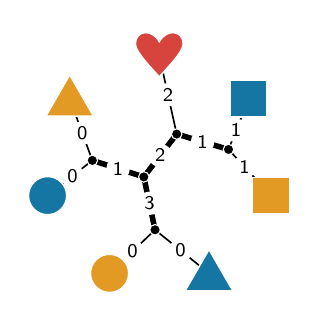
\begin{tikzpicture}[x=1.0cm,y=1.0cm,baseline=(current bounding box.center)]
\coordinate (v1) at (1.13770,0.90728);
\coordinate (v2) at (0.63137,-1.31106);
\coordinate (v3) at (-1.41868,-0.32381);
\coordinate (v4) at (1.41868,-0.32381);
\coordinate (v5) at (-1.13770,0.90728);
\coordinate (v6) at (-0.63137,-1.31106);
\coordinate (v7) at (0.00000,1.45517);
\coordinate (v8) at (-0.05387,-0.75780);
\coordinate (v9) at (0.87924,0.26266);
\coordinate (v10) at (0.22128,0.45821);
\coordinate (v11) at (-0.85011,0.12332);
\coordinate (v12) at (-0.19653,-0.08639);
\draw[g2tree internal] (v8)--(v12);
\draw[g2tree internal] (v9)--(v10);
\draw[g2tree internal] (v10)--(v12);
\draw[g2tree internal] (v11)--(v12);
\draw[g2tree pendant] (v1)--(v9);
\draw[g2tree pendant] (v2)--(v8);
\draw[g2tree pendant] (v3)--(v11);
\draw[g2tree pendant] (v4)--(v9);
\draw[g2tree pendant] (v5)--(v11);
\draw[g2tree pendant] (v6)--(v8);
\draw[g2tree pendant] (v7)--(v10);
\node[g2tree weight,font={\sffamily\fontsize{7.5}{8}\selectfont}] at (-0.12520,-0.42209) {3};
\node[g2tree weight,font={\sffamily\fontsize{7.5}{8}\selectfont}] at (0.55026,0.36043) {1};
\node[g2tree weight,font={\sffamily\fontsize{7.5}{8}\selectfont}] at (0.01237,0.18591) {2};
\node[g2tree weight,font={\sffamily\fontsize{7.5}{8}\selectfont}] at (-0.52332,0.01846) {1};
\node[g2tree weight,font={\sffamily\fontsize{7.5}{8}\selectfont}] at (0.97616,0.50439) {1};
\node[g2tree weight,font={\sffamily\fontsize{7.5}{8}\selectfont}] at (0.27062,-1.01979) {0};
\node[g2tree weight,font={\sffamily\fontsize{7.5}{8}\selectfont}] at (-1.10197,-0.07474) {0};
\node[g2tree weight,font={\sffamily\fontsize{7.5}{8}\selectfont}] at (1.08153,0.04274) {1};
\node[g2tree weight,font={\sffamily\fontsize{7.5}{8}\selectfont}] at (-0.97801,0.47198) {0};
\node[g2tree weight,font={\sffamily\fontsize{7.5}{8}\selectfont}] at (-0.34043,-1.03233) {0};
\node[g2tree weight,font={\sffamily\fontsize{7.5}{8}\selectfont}] at (0.11064,0.95669) {2};
\node[g2tree vertex] at (v8) {};
\node[g2tree vertex] at (v9) {};
\node[g2tree vertex] at (v10) {};
\node[g2tree vertex] at (v11) {};
\node[g2tree vertex] at (v12) {};
\node[g2tree dark,rectangle,minimum size=4.657500000000001mm,font={\sffamily\fontsize{9}{9}\selectfont\bfseries}] at (v1) {};
\begin{scope}[shift={(v2)},scale=1.0125000000000002,transform shape]
\path[fill=g2TaxonBlue,draw=white,line width=.55pt,line join=round] (0mm,3.0mm)--(-3.0mm,-2.2mm)--(3.0mm,-2.2mm)--cycle;
\end{scope}
\node[g2tree dark,circle,minimum size=4.86mm,font={\sffamily\fontsize{9}{9}\selectfont\bfseries}] at (v3) {};
\node[g2tree light,rectangle,minimum size=4.657500000000001mm,font={\sffamily\fontsize{9}{9}\selectfont\bfseries}] at (v4) {};
\begin{scope}[shift={(v5)},scale=1.0125000000000002,transform shape]
\path[fill=g2TaxonYellow,draw=white,line width=.55pt,line join=round] (0mm,3.0mm)--(-3.0mm,-2.2mm)--(3.0mm,-2.2mm)--cycle;
\end{scope}
\node[g2tree light,circle,minimum size=4.86mm,font={\sffamily\fontsize{9}{9}\selectfont\bfseries}] at (v6) {};
\begin{scope}[shift={(v7)},scale=1.0125000000000002,transform shape]
\path[fill=g2HeartRed,draw=white,line width=.55pt]
  (0mm,-2.7mm)..controls(-.45mm,-2.1mm)and(-3.0mm,.35mm)..(-3.0mm,1.45mm)
  ..controls(-3.0mm,3.2mm)and(-.9mm,3.4mm)..(0mm,1.75mm)
  ..controls(.9mm,3.4mm)and(3.0mm,3.2mm)..(3.0mm,1.45mm)
  ..controls(3.0mm,.35mm)and(.45mm,-2.1mm)..(0mm,-2.7mm)--cycle;
\end{scope}
\end{tikzpicture}
\endgroup
\par}
\vskip 0pt plus 1filll
\noindent\rlap{char\ 2}\par
\end{minipage}
\\
\end{tabular}
\endgroup
